\chapter{Results}
\label{chap:results}
In the last chapter, we discussed the implementation of our method. In this chapter, we are going to check it after the assumptions we stated in chapter \ref{chap:intro}, discussing advantages, disadvantages, and trade-offs. In the first section, we will discuss the quality result of our method, comparing it to path-traced results. In the second section, we will discuss how close we can get to the expected results in the performance domain, testing it for different parameters. 

\section{Parameters}
\label{sec:parameters}
The parameters were introduced in the previous chapter \ref{chap:implementation}. We will sum them up here, in order to have a reference for this chapter.

\begin{itemize}
\item $M$, the total number of points in the disk. We recall that we make a disc of the size of the object bounding box and then generate $M$ exponentially based samples in it. Unless otherwise stated, $M = 1000$
\item $q$, the modifier of the exponential distribution of the samples. Unless otherwise stated, $q = 1$. 
\item $N$, the number of samples used from the disc. It is always $N < M$.
\item $K$, the number of directions used in the radiance map. Unless otherwise stated, $K = 16$. 
\item $L$, the number of lights in the scene. 
\item $W_l$, the size in pixel of the light map. Unless otherwise stated, $W_l = 512$.
\item $W_r$, the size in pixel of the radiance map. Unless otherwise stated, $W_r = 1024$.
\end{itemize}

Other parameters are available in the method, such as all the parameters of the cameras. In this section, we listed only the parameters that makes sense for the user to tweak, and that can directly influence the quality or the performance of the final result.

\section{Quality comparisons}

In the domain of quality, we compared our method to offline rendered solutions, always made using the directional dipole. The solutions are compared only visually, since if was not possible to perfectly match the perspective and view cameras of the original pictures. We will see that the visual results of our method, given enough samples, can produce a result comparable to the one of a offline rendered solution. We will compare our results at convergence (after 100 frames of evolution), unless otherwise stated.

\subsection{Optimal radius}
\label{sec:radius}
In section \ref{sec:exponentiallybiased}, we discussed how to generate exponentially biased points in our implementation. In our algorithm, to choose how to distribute the sampling points, we adopt the strategy of choosing a distribution biased towards the following exponent:
$$
\sigma^* = \frac{\min(\sigma_{tr,x},\sigma_{tr,y},\sigma_{tr,z})}{q}
\label{eq:moo}
$$
We can see why we use the minimum coefficient in Figures \ref{fig:radiuscolor} and \ref{fig:Bunnytr}. $\sigma_{tr}$ as a coefficient, is related to how much the scattering effects propagate. If we look at the directional dipole formula in \ref{eq:dirdipole}, we can see that the dipole has a leading term depending on $e^{-\sigma_{tr} t}$. If we consider only this term, the average distance the light travels in the medium is $1/\sigma_{tr}$. Figure \ref{fig:radiuscolor} shows these radii for the potato and the ketchup material. So, in order to account for all channels in our sampling, we need choose as a exponent for our sampling pdf the maximum radius:
$$
\max\left(\frac{1}{\sigma_{tr,x}},\frac{1}{\sigma_{tr,y}},\frac{1}{\sigma_{tr,z}}\right) = \min(\sigma_{tr,x},\sigma_{tr,y},\sigma_{tr,z})
$$
And this is how we obtain Equation \ref{eq:moo}. We will see in the next section that the $q$ parameter in the equation is necessary in order to allow better performance with a fewer number of samples. In Figure \ref{fig:Bunnytr} we can see the effects of choosing different radii according to the three coefficients in ketchup. When we use the red radius, all the effects are accounted for. When we use the green radius, we lose the red absorption part. If we use the blue channel, the green and the red part of the absorption spectrum disappear, resulting in a gray/blue appearance.

\begin{figure}[h]
\centering
\subfloat[Potato]{
  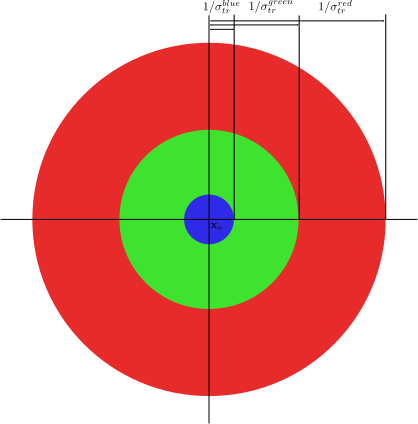
\includegraphics[width=0.5\linewidth]{images/radius_potato}
}
\subfloat[Ketchup]{
  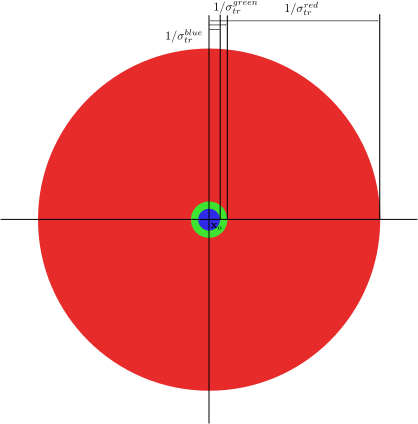
\includegraphics[width=0.5 \linewidth]{images/radius_ketchup}
}
\caption{Average radius of which the scattering effects are important for ketchup and potato materials.}
\label{fig:radiuscolor}
\end{figure}

\begin{figure}[h]
\centering
\subfloat[{$\sigma^* = \sigma_{tr,x}$}]{
  \includegraphics[width=0.33 \linewidth]{images/results/Bunny_tr0.png}
}
\subfloat[{$\sigma^* = \sigma_{tr,y}$}]{
  \includegraphics[width=0.33 \linewidth]{images/results/Bunny_tr1.png}
}
\subfloat[{$\sigma^* = \sigma_{tr,z}$}]{
  \includegraphics[width=0.33 \linewidth]{images/results/Bunny_tr2.png}
}
\caption{Bunny rendered with different radii. We can appreciate the different absorptions according to the distribution radius. $N = 20$, $M = 160$, $q = 1$ in all images.}
\label{fig:Bunnytr}
\end{figure}

\subsection{Tests with different number of samples}

The material tested where:
\begin{itemize}
	\item  Potato, a highly scattering isotropic material ($\alpha = \sigma_s / \sigma_a \approx 10^2$), 
	\item  Marble, a even higher high scattering material ($\alpha \approx 10^4$) 
	\item  White grapefruit juice, a material with a big forward scattering component ($\alpha \approx 10^2$, $g \approx 0.5$)
	\item  Ketchup, a material that has a strong absorption component in the red channel ($\alpha_{red} \approx 10^{-2}$, $\alpha_{green} \approx \alpha_{blue} \approx 10^2$)
	\item  Beer, a high absorption material with nearly no scattering.
\end{itemize}
We are biased against highly scattering material because those are the material where our BSSRDF model gives our best results. However, we included materials as beer and ketchup to provide a comparison of our method even where the original BSSRDF model should fail.

The first comparison we make is with the path traced spheres generated in Figure \ref{fig:examplesmaterials}. The results are illustrated in Figure \ref{fig:pathpotato}, comparing different values of $M$ and $N$ for a potato sphere. We can see that different values of $M$ and $N$ greatly influence the results. In fact, for a big $M$ and the same $N$, the samples tend to be closer to the exiting point $x_o$, so the results are more accurate on the highlight region. If instead we chose a relatively small $M$, the points are widely spread on the surface, to the absorption of the material is accounted for more. This results in a sphere with gradients that are closer to the reference. In this case, the highlights are way more difficult to see. 

The result that gets closer to the reference solution is the one where $N = M = 1000$, but as we will see this values are unfeasible in the realm of performance, even for simple models. So, it is the artist that should find the right balance between $M$ and $N$ in order to get a satisfying result. 

\begin{figure}
\centering
\subfloat[{$N = 120$, $M = 120$}]{
  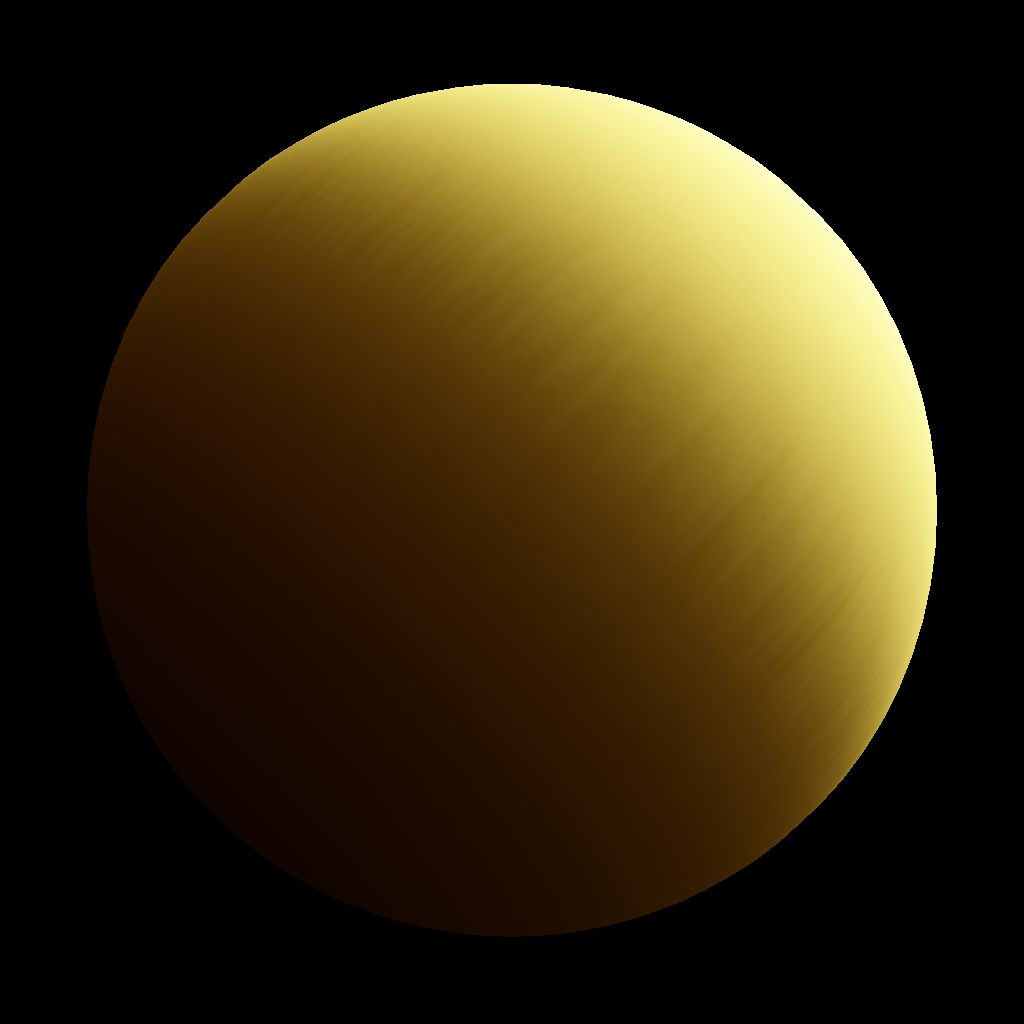
\includegraphics[width=0.33 \linewidth]{images/results/test_120_over_120.png}
}
\subfloat[{$N = 120$, $M = 300$}]{
  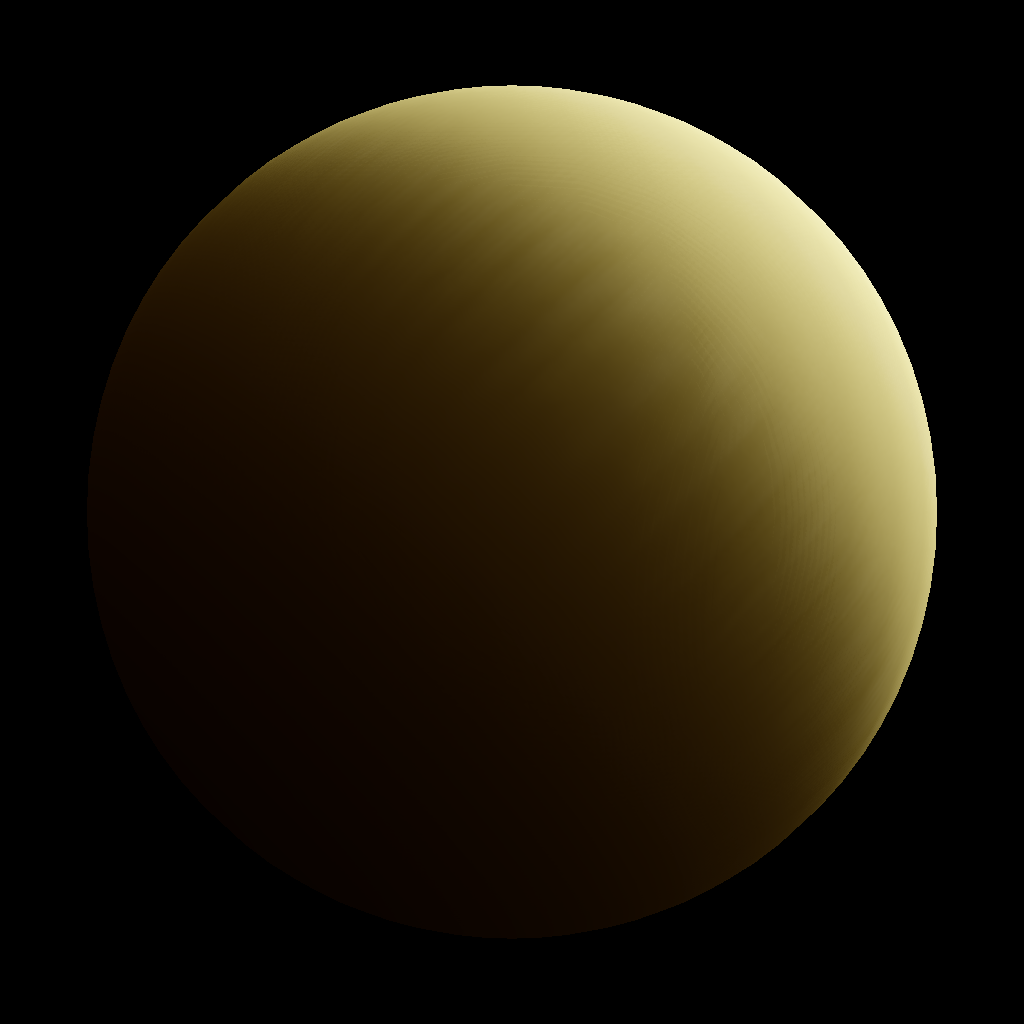
\includegraphics[width=0.33 \linewidth]{images/results/test_120_over_300.png}
}
\subfloat[{$N = 300$, $M = 300$}]{
  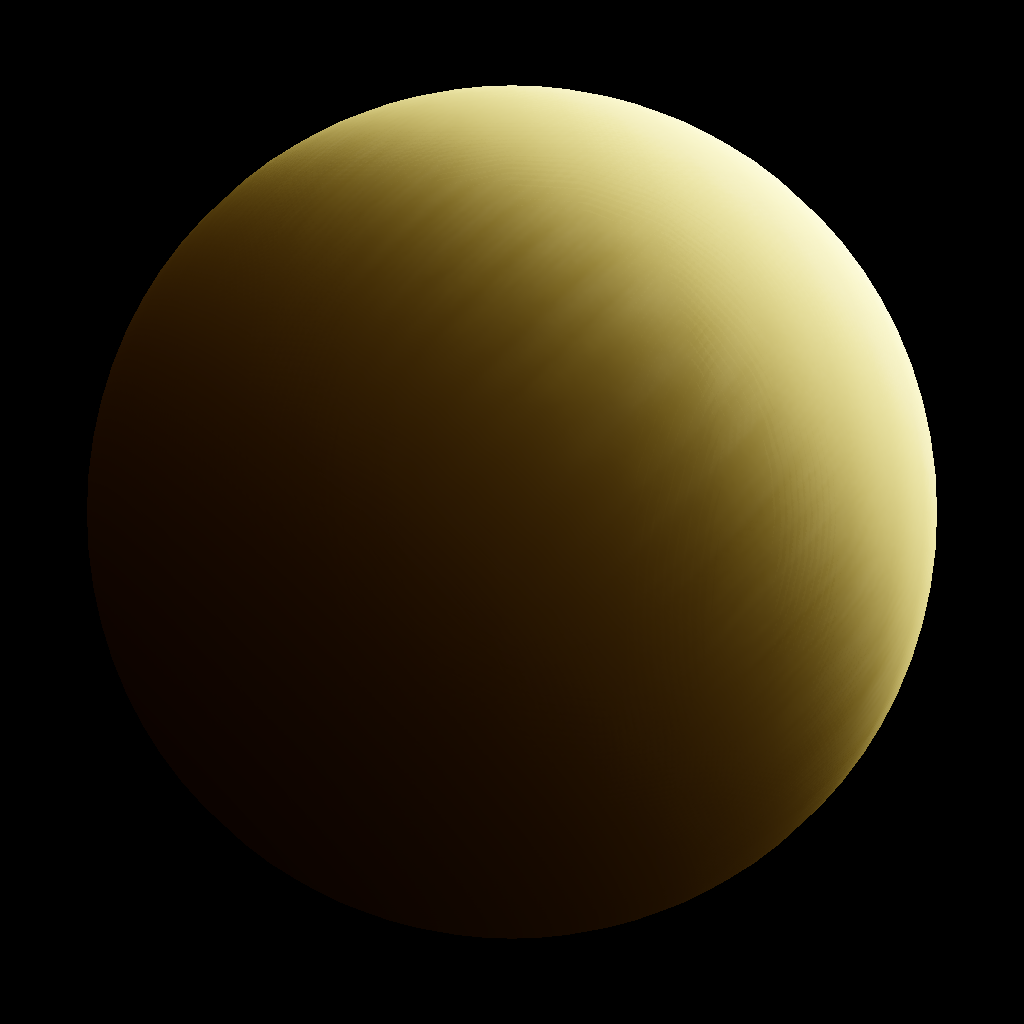
\includegraphics[width=0.33 \linewidth]{images/results/test_300_over_300.png}
} \\
\subfloat[{$N = 120$, $M = 1000$}]{
  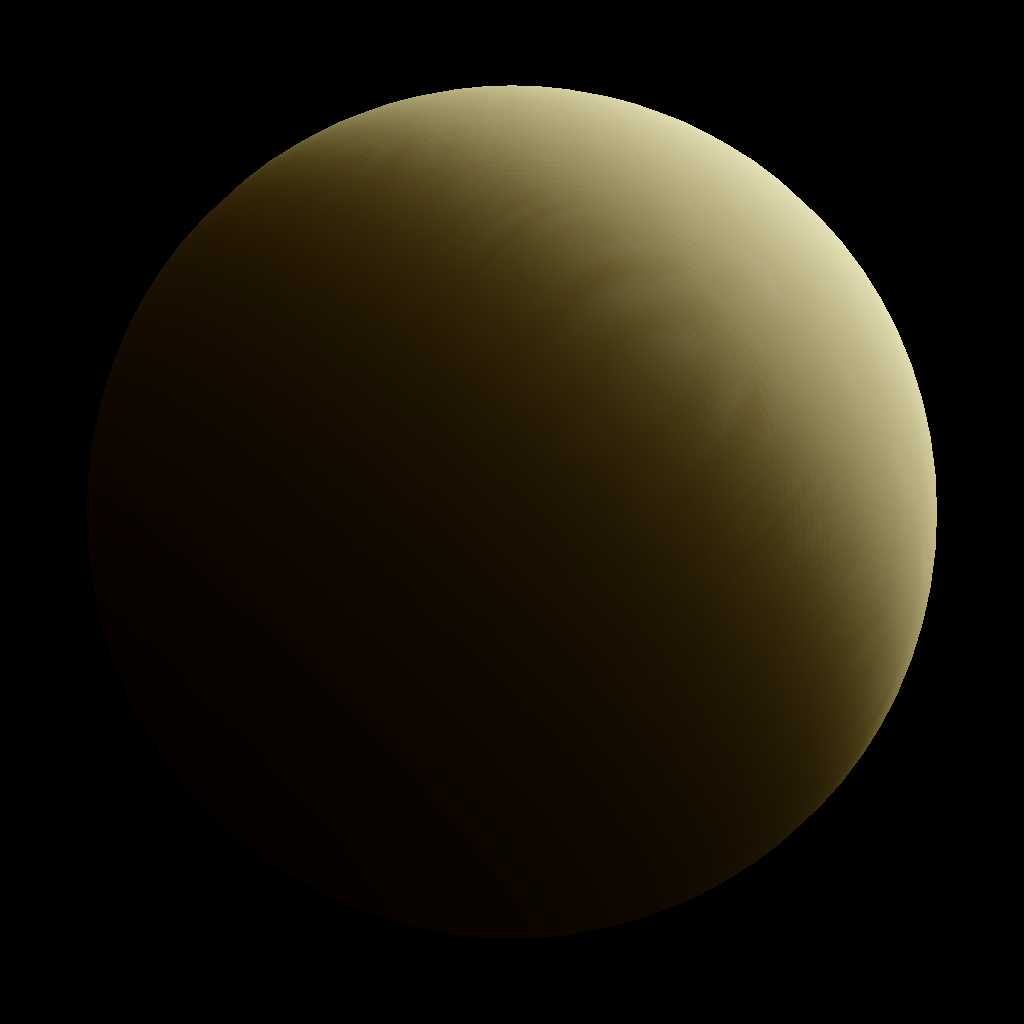
\includegraphics[width=0.33 \linewidth]{images/results/test_120_over_1000.png}
}
\subfloat[{$N = 300$, $M = 1000$}]{
  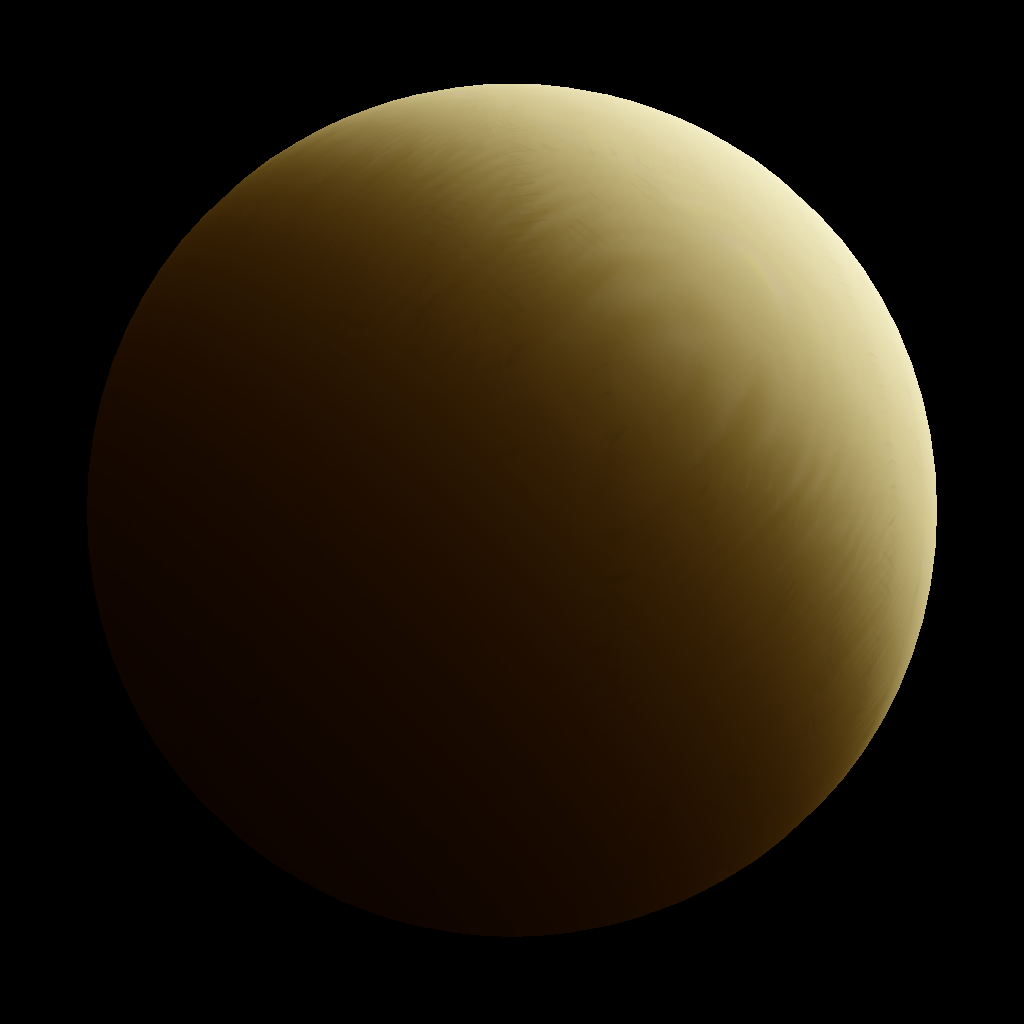
\includegraphics[width=0.33 \linewidth]{images/results/test_300_over_1000.png}
}
\subfloat[{$N = 1000$, $M = 1000$}]{
  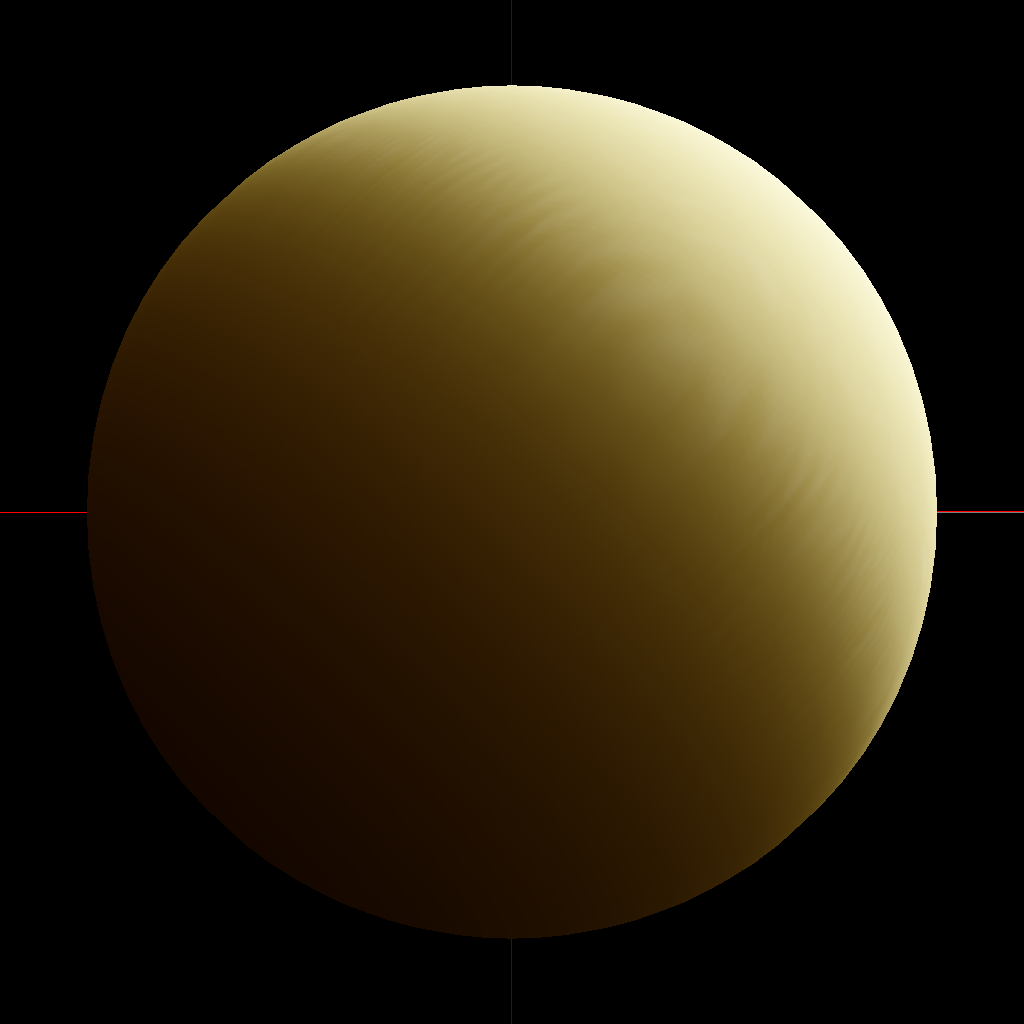
\includegraphics[width=0.33 \linewidth]{images/results/test_1000_over_1000.png}
} \\
\subfloat[Path traced solution]{
  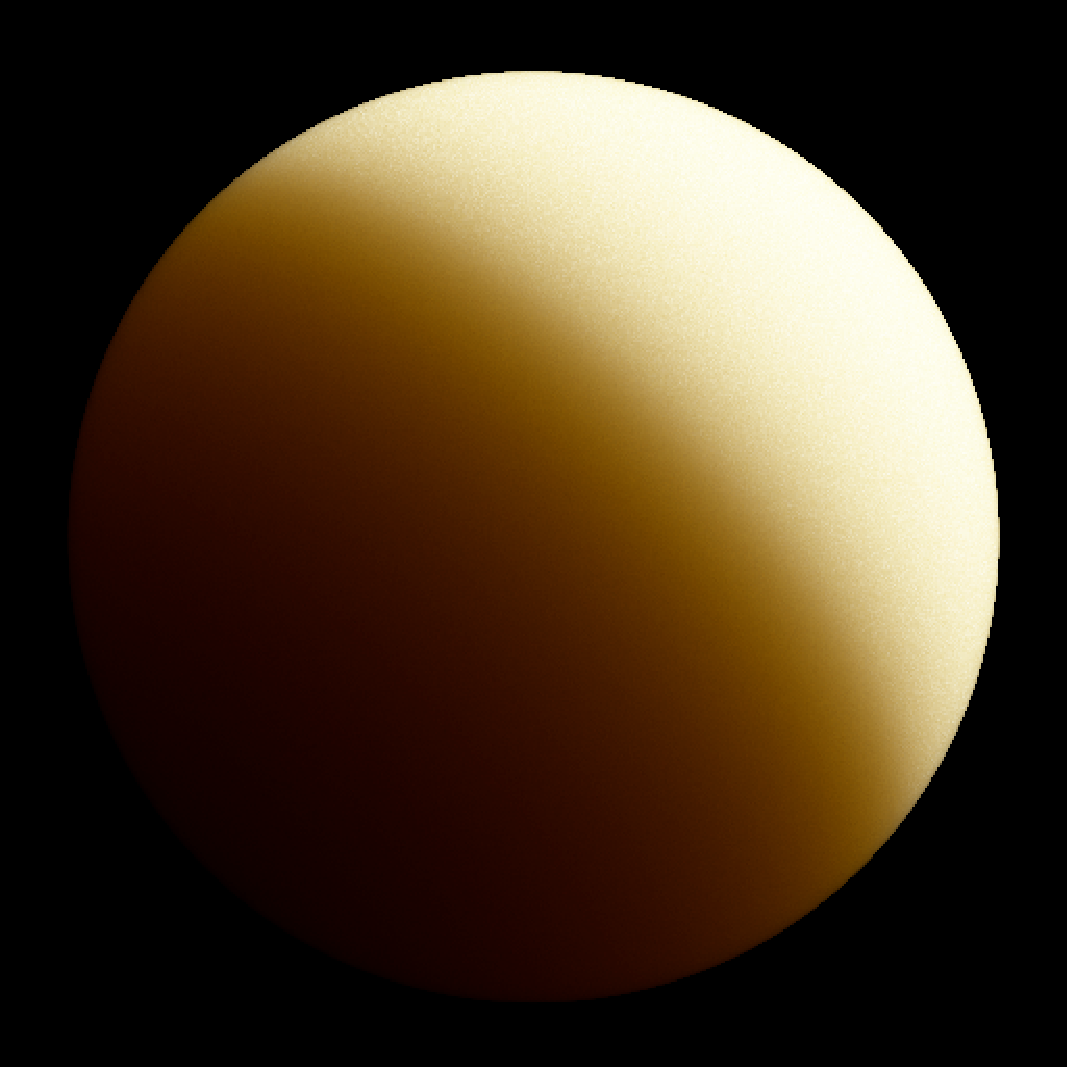
\includegraphics[width=0.33 \linewidth]{images/pathtrace/image-potato.pdf}
}
 \\
\caption{Path traced rendering on a sphere of potato material compared with the results of our method. The parameters are from table \ref{table:scatteringcoefficients}.}
\label{fig:pathpotato}
\end{figure}
 
In the next set of experiments, we can see the utility of the $q$ parameter. We tested a sphere of white grapefruit juice in Figure \ref{fig:pathgrapefruit}, a material with a high forward scattering component. In this case we can see that that with a smaller number of samples $N = 100$ and a $q = 3$ we can approximate very well the solution where $N = 1000$ and $q = 1$, way more expensive for the GPU. In a test with marble, in Figure \ref{fig:pathmarble} we can see that our sampling introduces artifacts, especially on the color transition area. In this case, $q$ slightly relieves the artifacts generated from the sampling.

\begin{figure}
\centering
\subfloat[{$N = 100$, $M = 1000$, $q = 1$}]{
  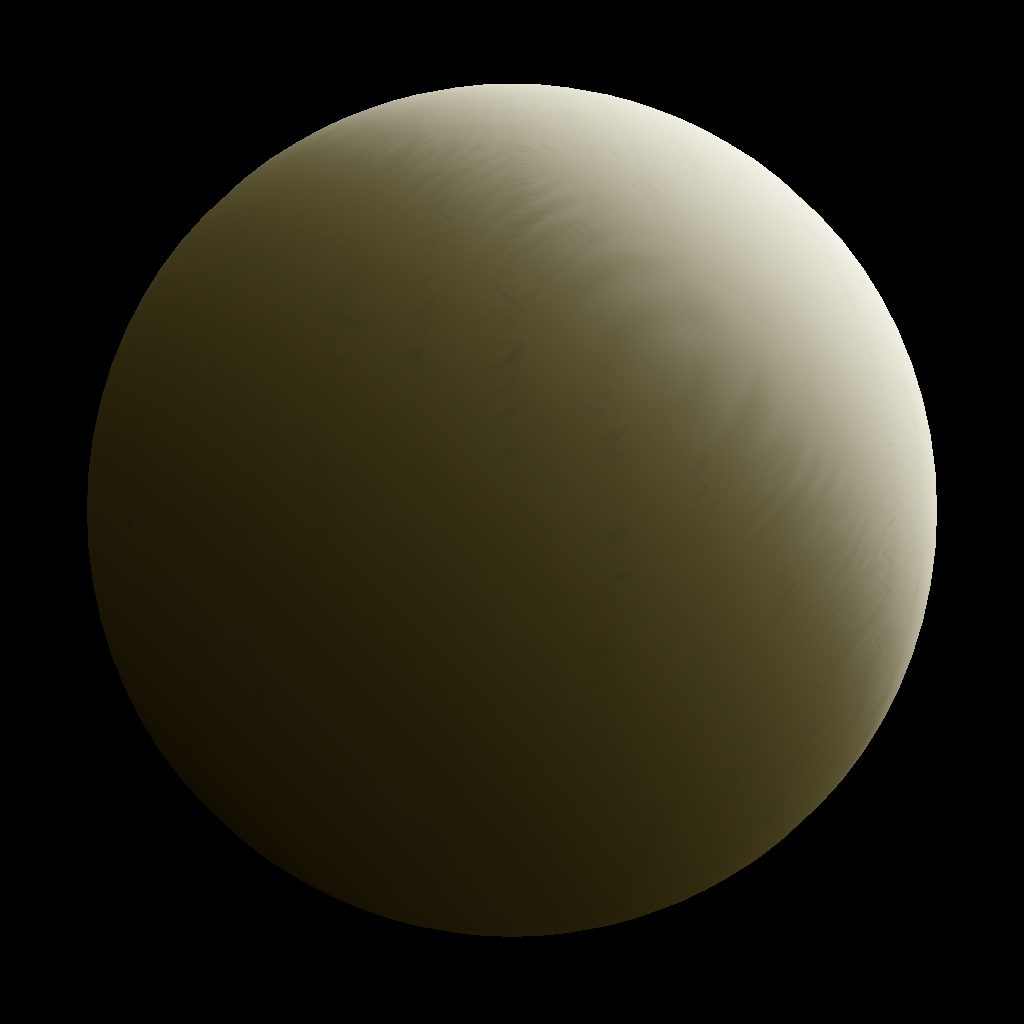
\includegraphics[width=0.5 \linewidth]{images/results/grapefruit_juice_comparison_100_over_1000_nobias.png}
}
\subfloat[{$N = 100$, $M = 1000$, $q = 3$}]{
  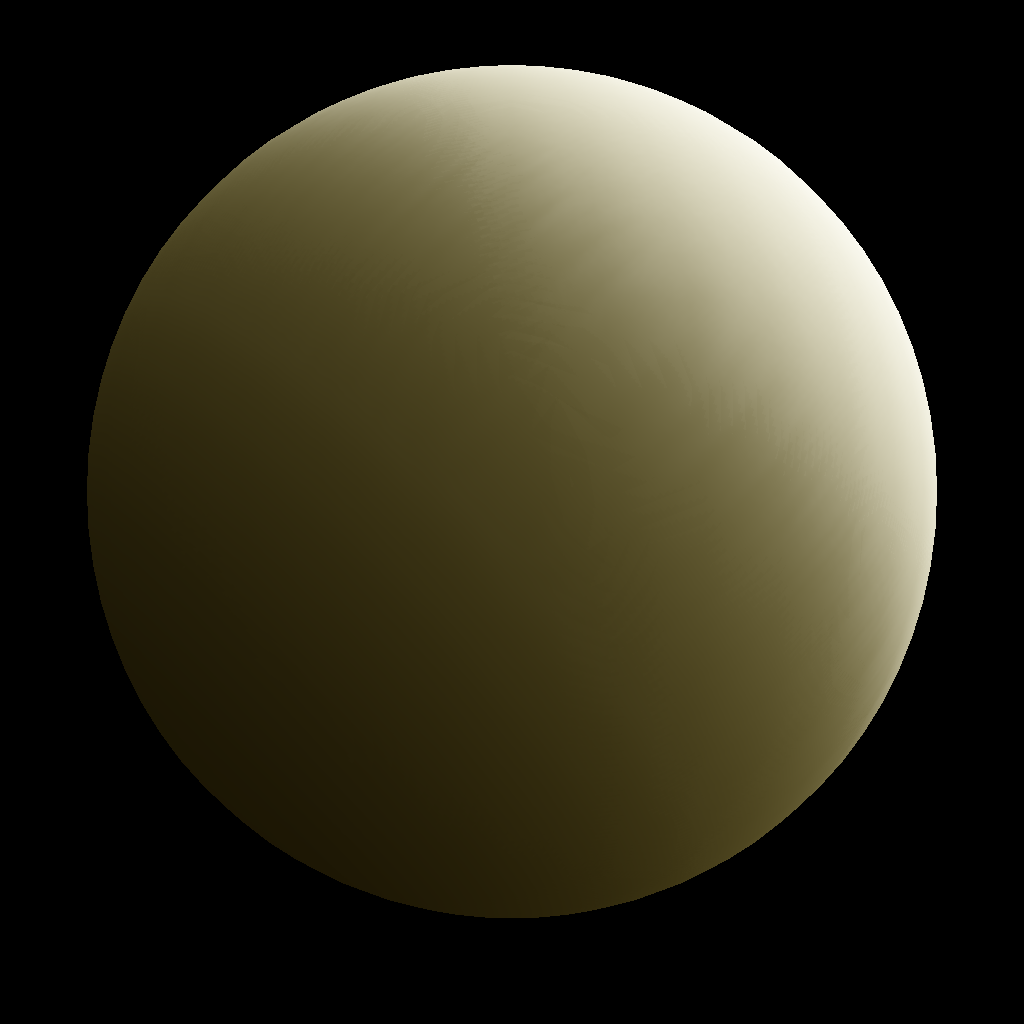
\includegraphics[width=0.5 \linewidth]{images/results/grapefruit_juice_comparison_100_over_1000_bias3.png}
}
\\
\subfloat[{$N = 1000$, $M = 1000$, $q = 1$}]{
  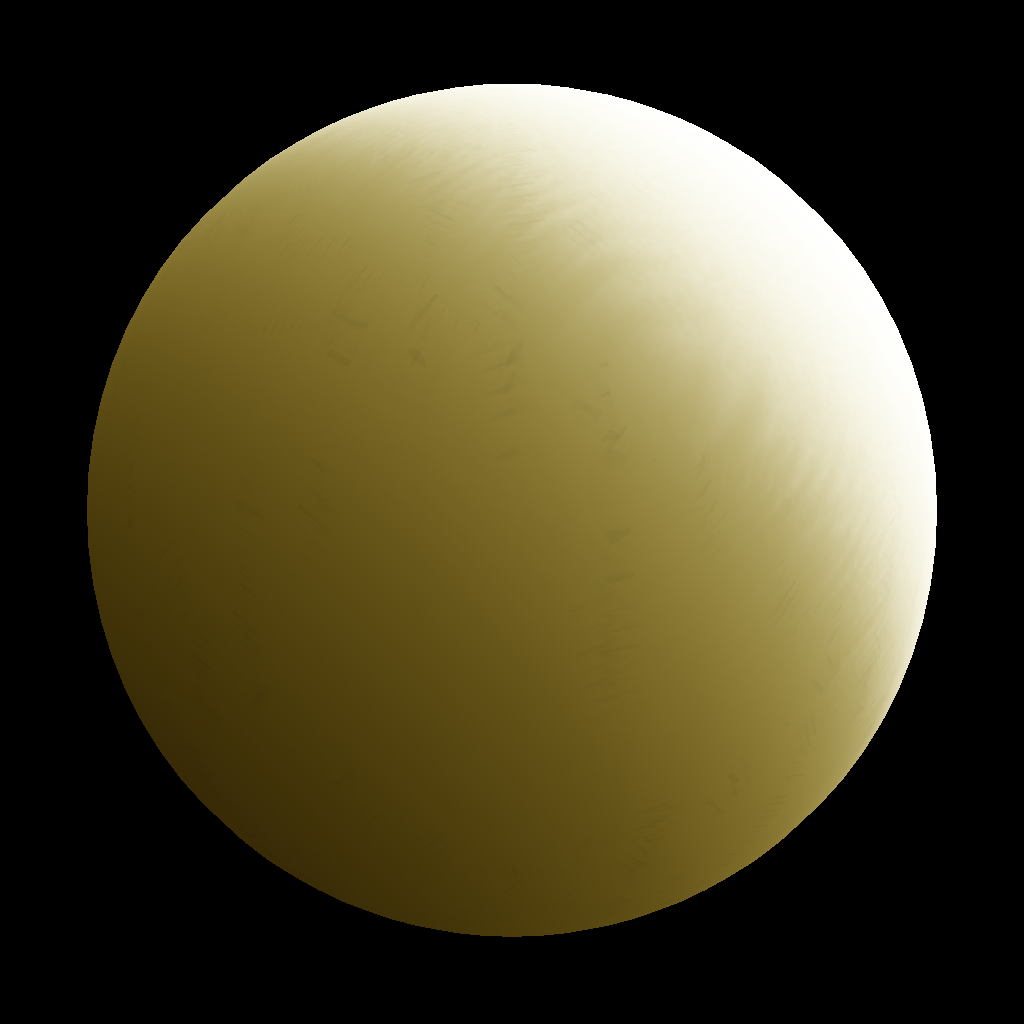
\includegraphics[width=0.5 \linewidth]{images/results/grapefruit_juice_comparison.png}
}
\subfloat[{Path traced result}]{
  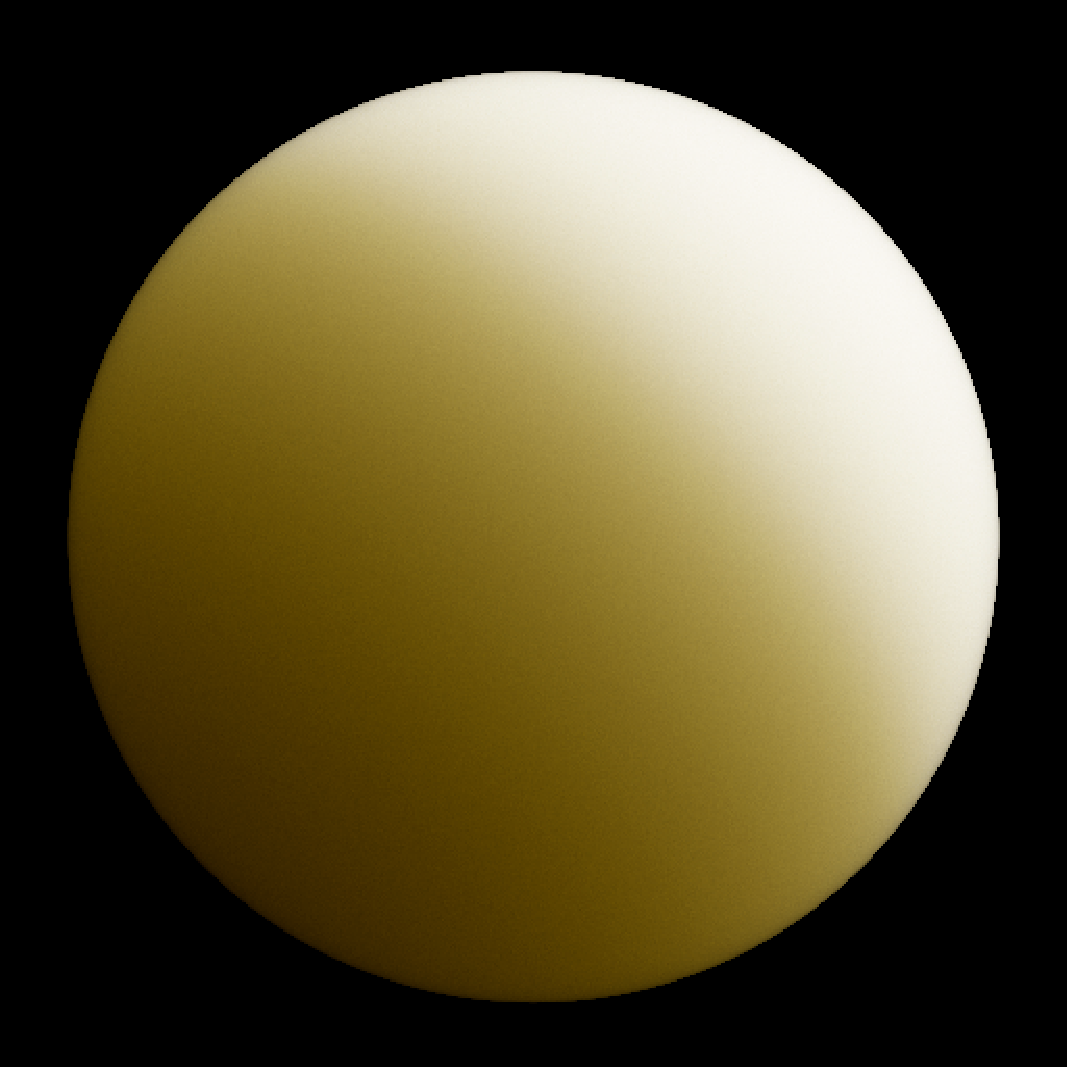
\includegraphics[width=0.5 \linewidth]{images/pathtrace/image-grapefruit.pdf}
}
\caption{Path traced rendering on a sphere of white grapefruit material compared with the results of our method. The parameters are from table \ref{table:scatteringcoefficients}. We can see that a higher $q$ helps us in approximating the path traced solution with fewer samples.}
\label{fig:pathgrapefruit}
\end{figure}

\begin{figure}
\centering
\subfloat[{$N = 120$, $M = 1000$, $q = 1.5$}]{
  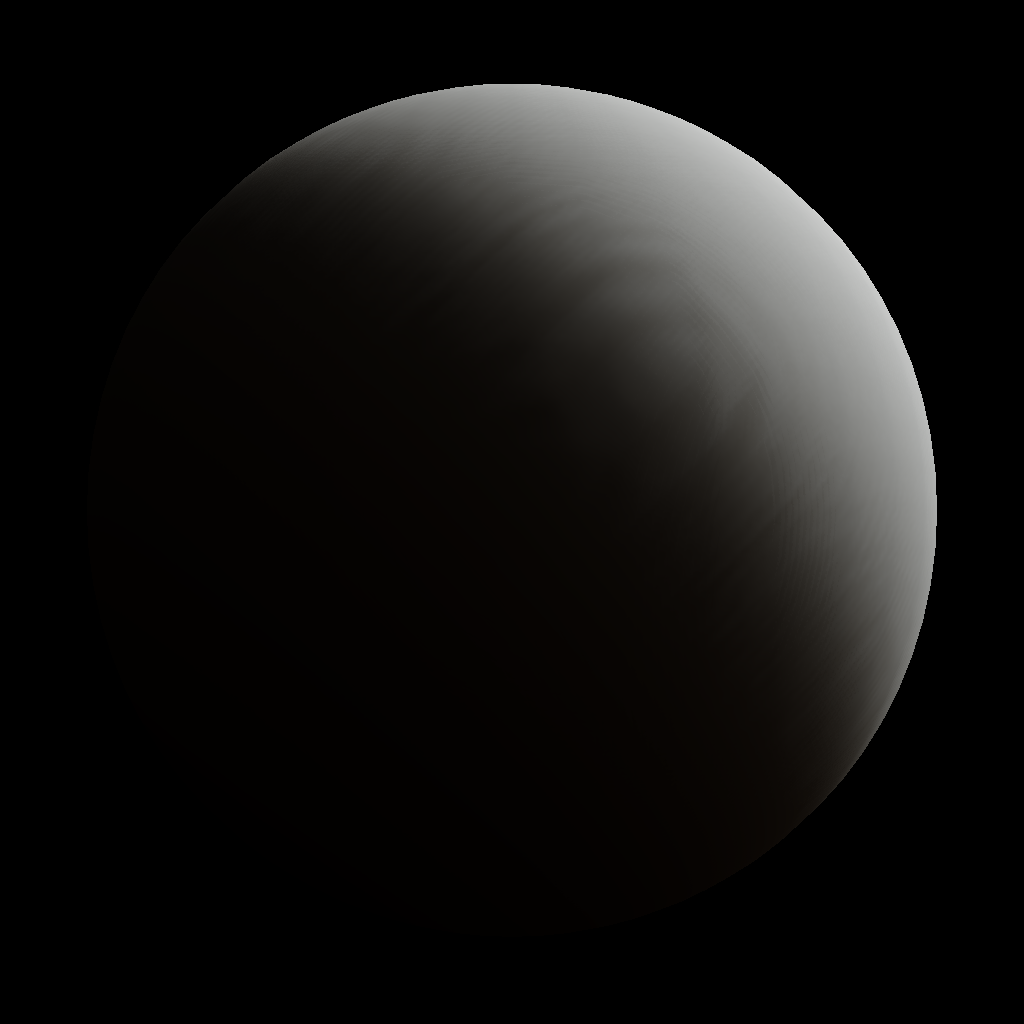
\includegraphics[width=0.4 \linewidth]{images/results/marble_120_over_1000_bias_1-5.png}
}
\subfloat[{$N = 120$, $M = 1000$, $q = 1$}]{
  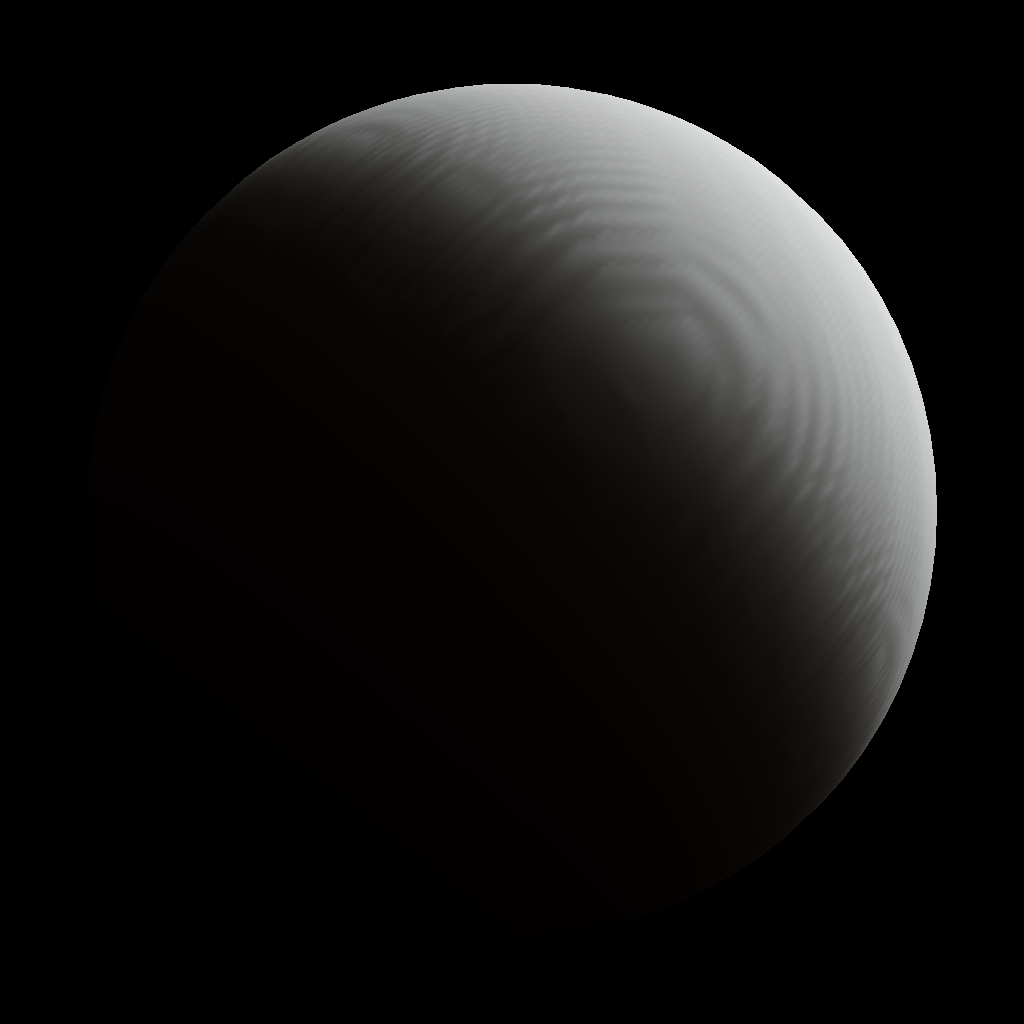
\includegraphics[width=0.4 \linewidth]{images/results/marble_120_over_1000_nobias.png}
}
\\
\subfloat[{$N = 1000$, $M = 1000$, $q = 1.5$}]{
  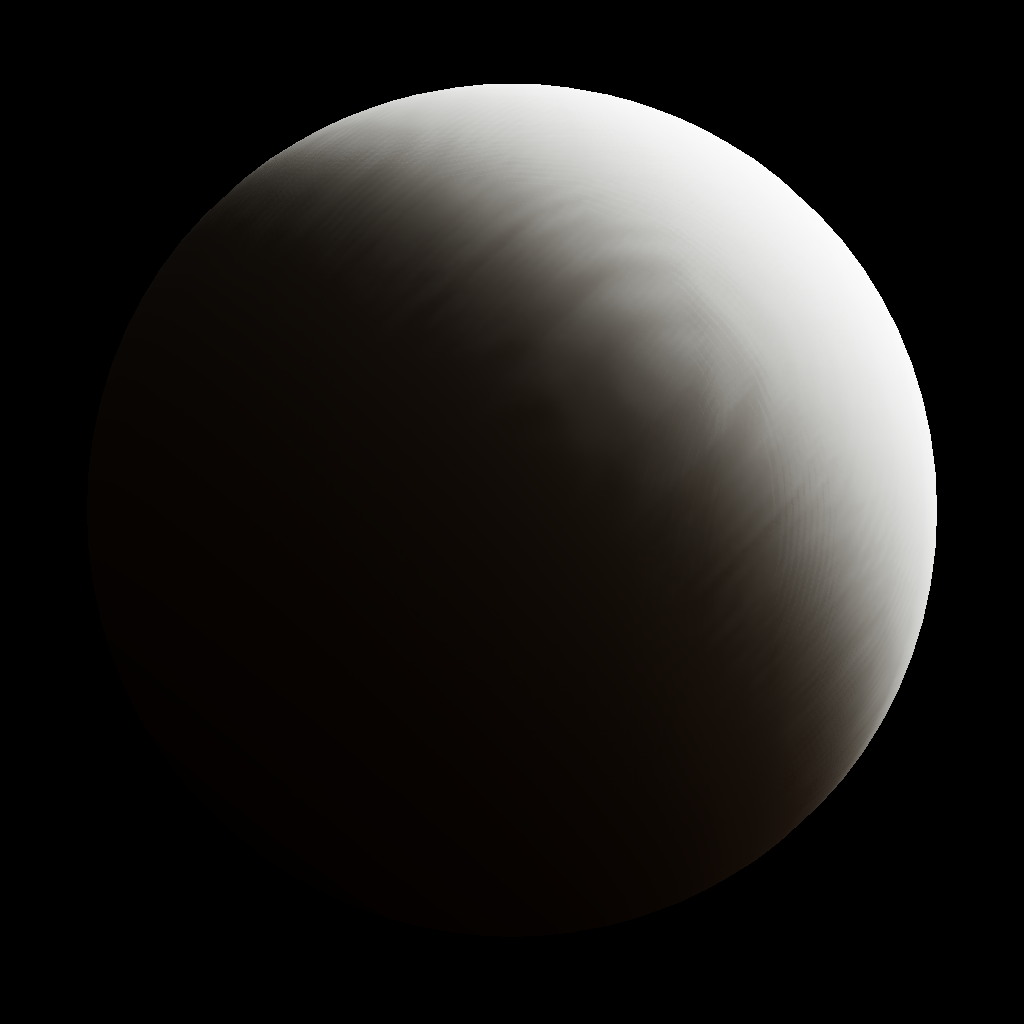
\includegraphics[width=0.4 \linewidth]{images/results/marble_1000_over_1000_bias_2.png}
}
\subfloat[{$N = 1000$, $M = 1000$, $q = 1$}]{
  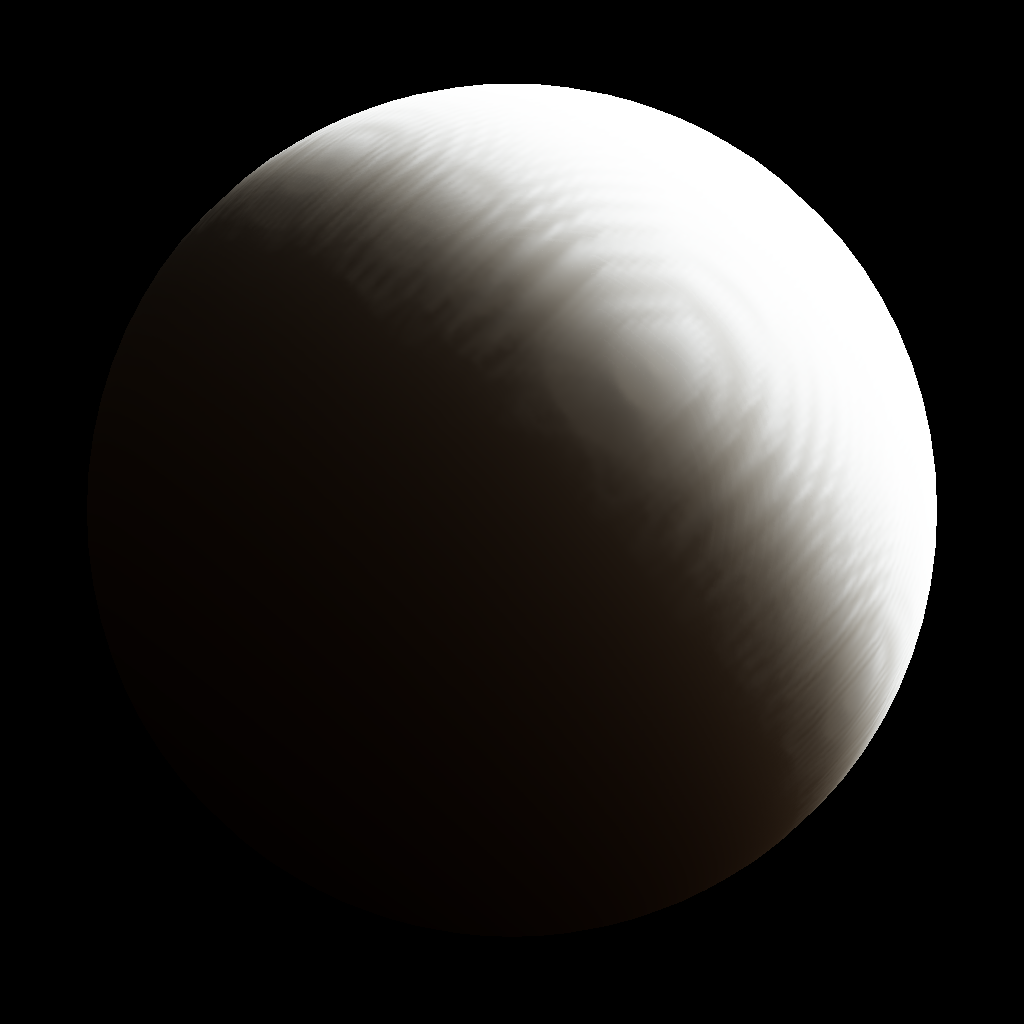
\includegraphics[width=0.4 \linewidth]{images/results/marble_1000_over_1000_biasno.png}
}
\\
\subfloat[{Path traced result}]{
  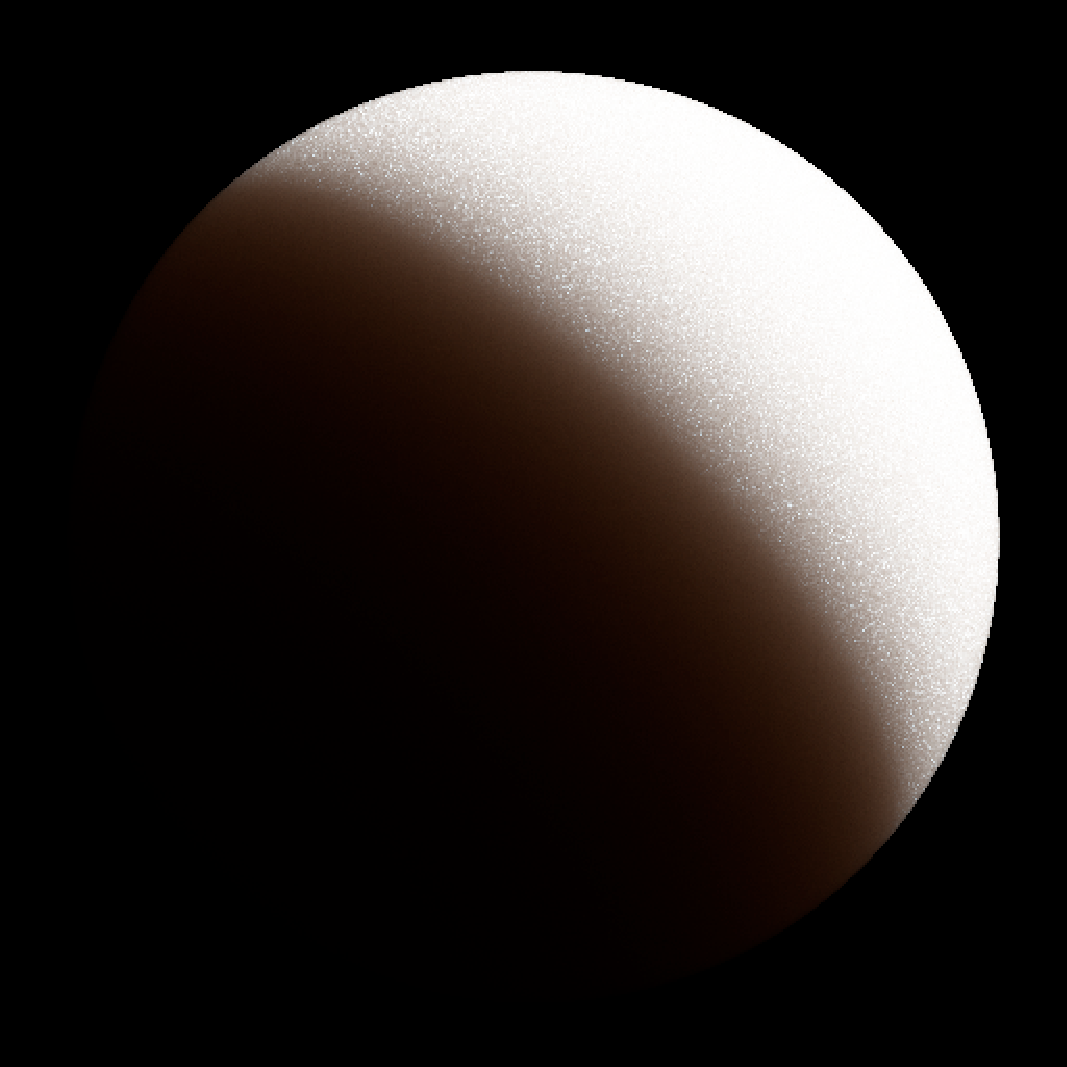
\includegraphics[width=0.4 \linewidth]{images/pathtrace/image-marble.pdf}
}
\caption{Path traced rendering on a sphere of marble material compared with the results of our method. The parameters are from table \ref{table:scatteringcoefficients}.}
\label{fig:pathmarble}
\end{figure}

\FloatBarrier
In Figure \ref{fig:pathbeer}, we can see a comparison between our method and a beer material: despite the obvious artifacts due to sampling, our results show a more realistic result that a path traced one. This happens because of the extremely low scattering coefficient of beer, that makes it unfeasible to use a Monte Carlo path tracer, since we need to sum a lot of contribution in order to remove all the noise. 

\begin{figure}[!ht]
\centering
\subfloat[{$N = 100$, $M = 100$, $q = 1$}]{
  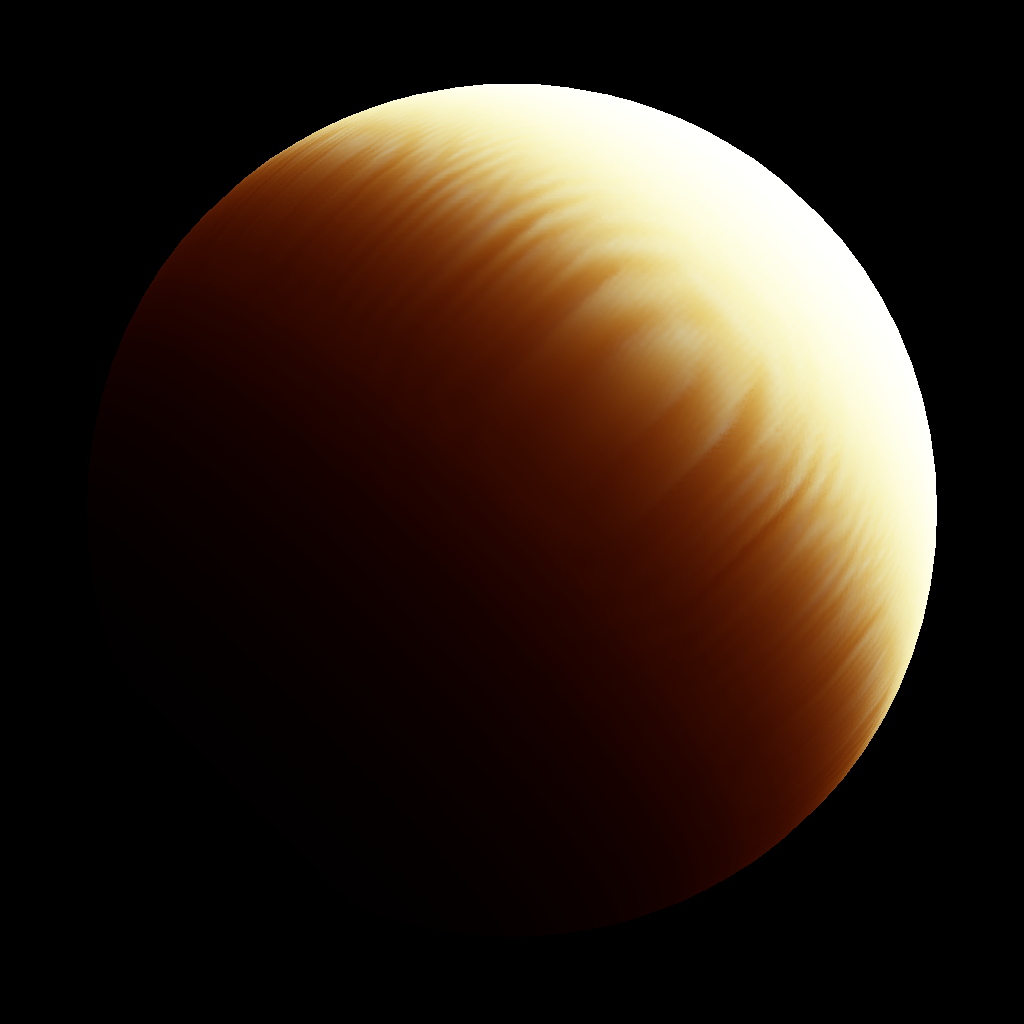
\includegraphics[width=0.5 \linewidth]{images/results/beer_100_over_100_no_bias.png}
}
\subfloat[{Path traced result}]{
  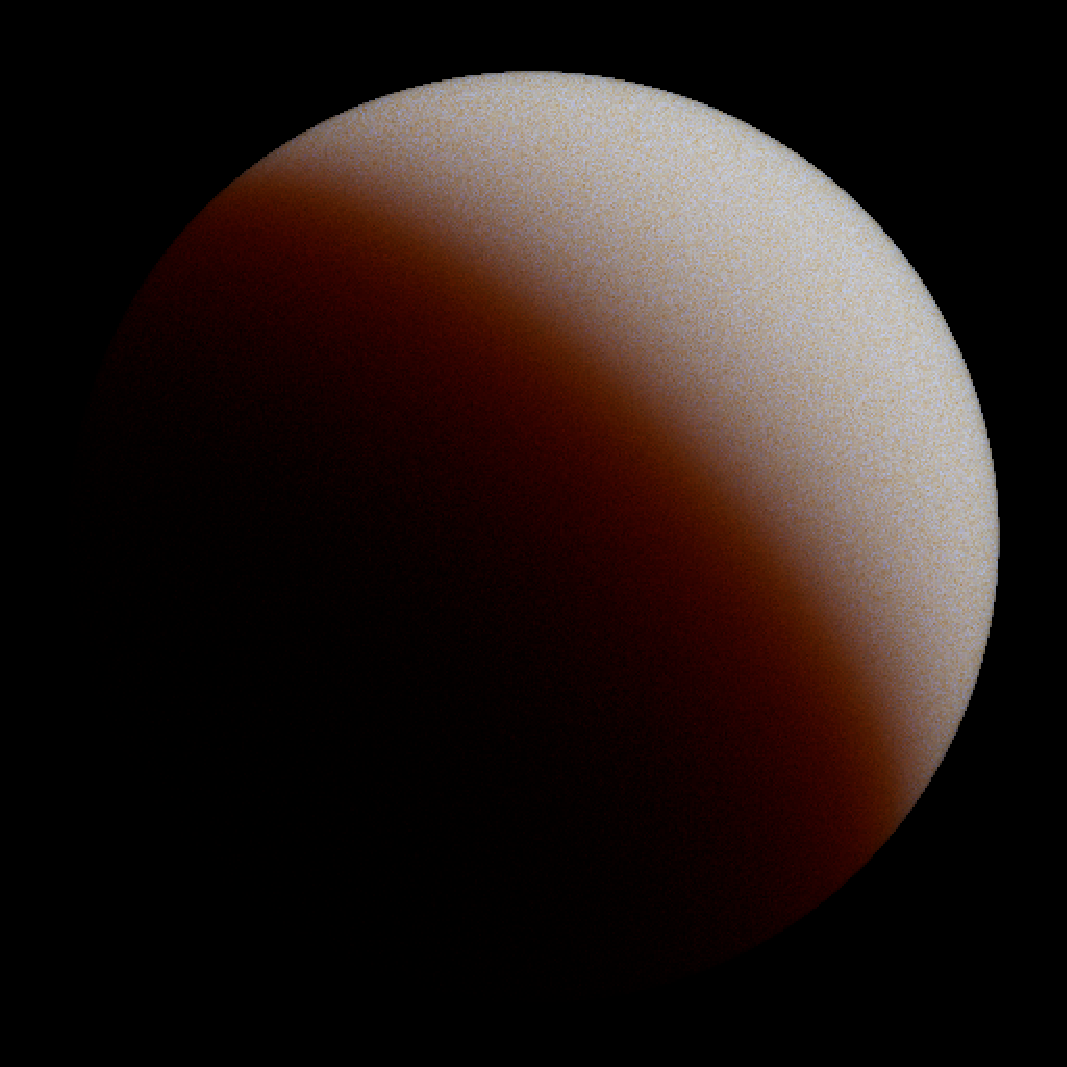
\includegraphics[width=0.5 \linewidth]{images/pathtrace/image-beer.pdf}
}
\caption{Path traced rendering on a sphere of beer material compared with the results of our method. The parameters are from table \ref{table:scatteringcoefficients}.}
\label{fig:pathbeer}
\end{figure}

The results that we obtained in the sphere renderings affect also the rendering of the full models. We tested a Buddha made of potato and a Dragon made of ketchup, that will be tested for performance in section \ref{sec:perf}. For the Buddha, we observe a slight color shift compared to reference as for the spheres in Figure \ref{fig:pathpotato}.

For the ketchup Dragon, instead, we observe that for a very low number of concentrated samples, the absorption contribution disappears, leaving only a gray scattering contribution that exhibits a pearling effect. If we reduce $M$, the highlights reduce and the absorption of the red part of the spectrum is accounted for.

\begin{figure}
\centering
\subfloat[{$N = 100$, $M = 1000$, $q = 1$}]{
  \includegraphics[width=0.333 \linewidth]{images/results/happy_Buddha_100_over_1000_nobias.png}
}
\subfloat[{$N = 200$, $M = 1000$, $q = 1$}]{
  \includegraphics[width=0.333 \linewidth]{images/results/happy_Buddha_200_over_1000_nobias.png}
}
\\
\subfloat[{$N = 100$, $M = 300$, $q = 1$}]{
  \includegraphics[width=0.333 \linewidth]{images/results/happy_Buddha_100_over_300_nobias.png}
}
\subfloat[{Path traced result}]{
  \includegraphics[width=0.333 \linewidth]{images/results/potato_Buddha_dir.png}
}
\caption{Rendering of a potato Buddha using the directional dipole, with increasing number of samples.}
\label{fig:pathBuddha}
\end{figure}

\begin{figure}
\centering
\subfloat[{$N = 10$, $M = 100$, $q = 1.5$}]{
  \includegraphics[width=0.5 \linewidth]{images/results/Dragon_10_over_100.png}
}
\subfloat[{$N = 50$, $M = 120$, $q = 1$}]{
  \includegraphics[width=0.5 \linewidth]{images/results/Dragon_50_over_120.png}
}
\\
\subfloat[{$N = 50$, $M = 1000$, $q = 1.5$}]{
  \includegraphics[width=0.5 \linewidth]{images/results/Dragon_50_over_1000_nobias.png}
}
\subfloat[{Path traced result}]{
  \includegraphics[width=0.5 \linewidth]{images/results/ketchup_Dragon_dir.png}
}
\label{fig:pathDragon}
\caption{Rendering of a ketchup Dragon using the directional dipole, with changing values of $M$ and $N$. }
\end{figure}

\clearpage
\subsection{Radiance map sizes tests}
Finally, we tested the effect of reducing the size of the texture used for the radiance map, for the Dragon test. As we can see, for diminishing values of $W_s$ the quality does not get too much worse until $W_s = 128$, where artifacts due to shadow mapping become evident, like bright seams and jagged pixels. In Figure \ref{fig:pathDragonsizett} the difference between the 1024 and the 256 image is reported. In the image, we can see that most of the difference are within $10\%$ of the high resolution value (since the image is enlarged 10 times and the full colored pixels are only a minority).

\begin{figure}[!h]
\centering
  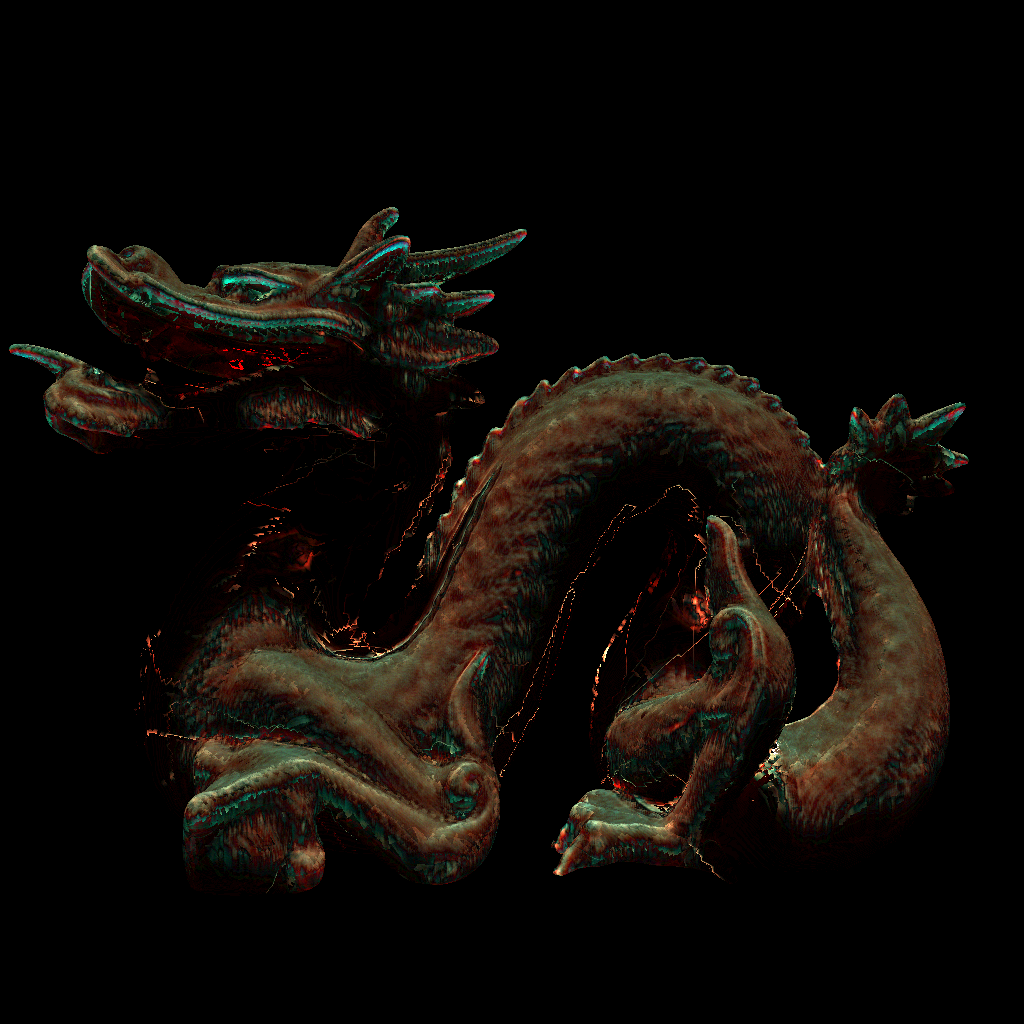
\includegraphics[width=0.7 \linewidth]{images/results/difference.png}
\caption{Difference multiplied by 10 times between \ref{fig:pathDragonsize1024} and \ref{fig:pathDragonsize256}.}
\label{fig:pathDragonsizett}
\end{figure}

\begin{figure}
\centering
\subfloat[{$W_s = 128$}]{
  \includegraphics[width=0.5 \linewidth]{images/results/Dragon_50_over_120_ws128.png}
}
\subfloat[{$W_s = 256$}]{
  \includegraphics[width=0.5 \linewidth]{images/results/Dragon_50_over_120_ws256.png}
	\label{fig:pathDragonsize256}
}
\\
\subfloat[{$W_s = 512$}]{
  \includegraphics[width=0.5 \linewidth]{images/results/Dragon_50_over_120_ws512.png}
	\label{fig:pathDragonsize512}
}
\subfloat[{$W_s = 1024$}]{
  \includegraphics[width=0.5 \linewidth]{images/results/Dragon_50_over_120_detail.png}
	\label{fig:pathDragonsize1024}
}
\label{fig:pathDragonsize}
\caption{Rendering of a ketchup Dragon using the directional dipole, with varying radiance map size $W_s$.}
\end{figure}

\FloatBarrier
\subsection{Tests of mipmap blurring quality}

In this part we tested the quality improvement from the mipmap blurring introduced in section \ref{sec:mipmaps} to the final image. We can see the result of our method at the first frame of our simulation for different mipmap levels. At the beginning of the evolution, a strong blurring (two passes) is needed to compensate the high level noise, as we can see from image \ref{fig:mipblurring}. During the evolution, a lesser level of mipmaps is needed in order to preserve a noiseless image. At convergence, we do not need mipmap blurring at all, as the result converge to the solution. 
\begin{figure}[!h]
\vspace{-0.5cm}
\centering
\subfloat[{Mipmap level 0 (no blur)}]{
  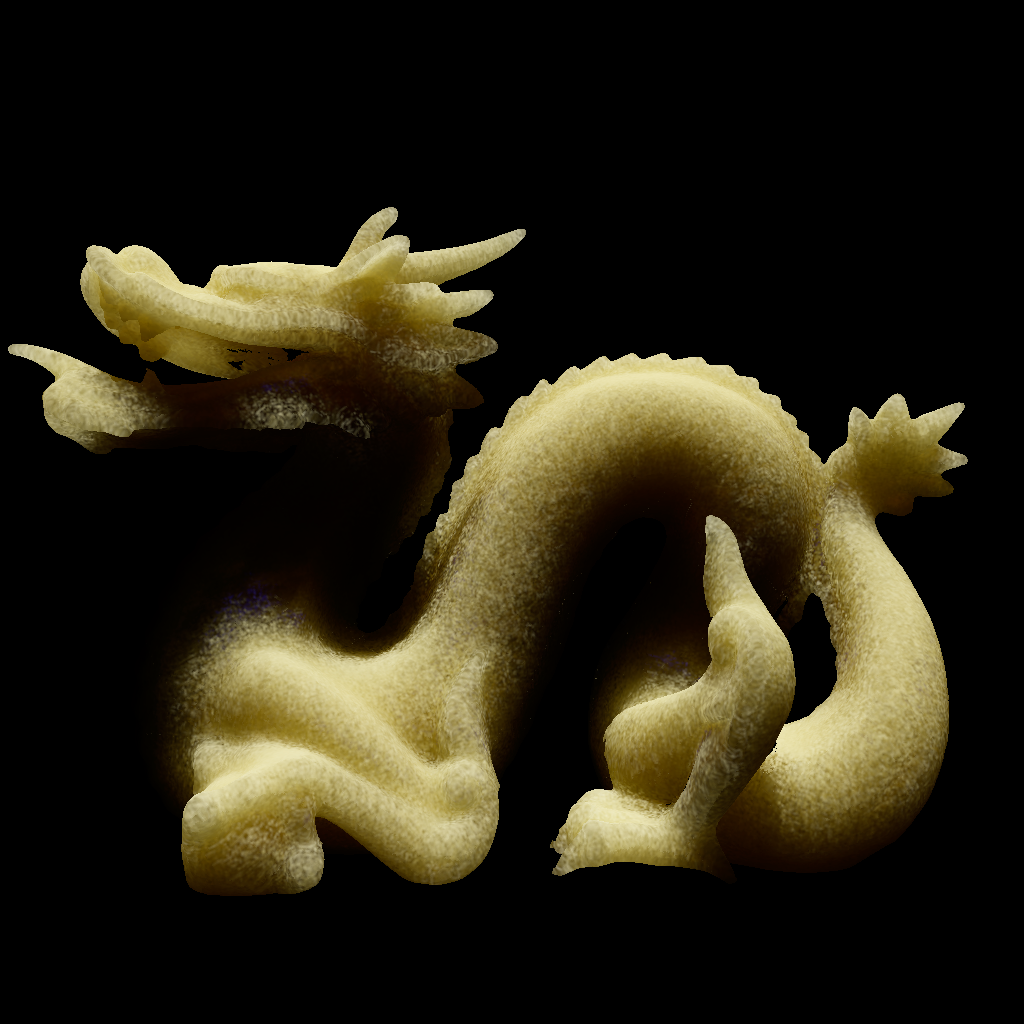
\includegraphics[width=0.4 \linewidth]{images/results/mipmaps00.png}
}
\subfloat[{Mipmap level 1}]{
  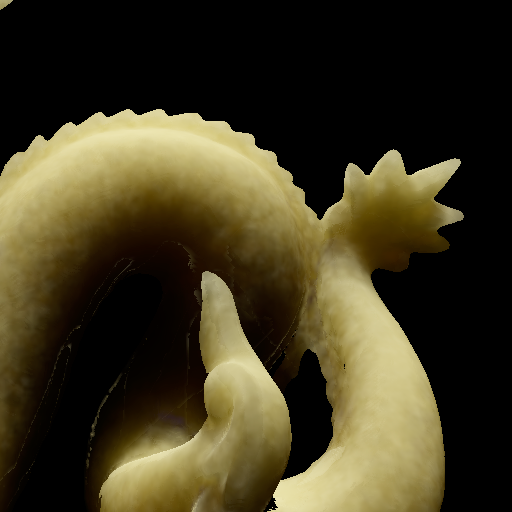
\includegraphics[width=0.4 \linewidth]{images/results/mipmaps01.png}
} \\

\subfloat[{Mipmap level 2}]{
  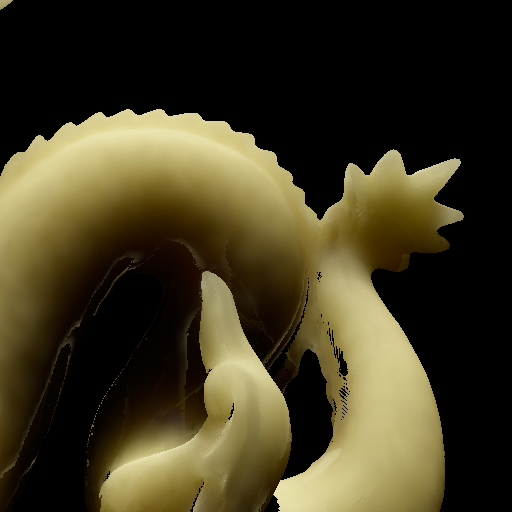
\includegraphics[width=0.4 \linewidth]{images/results/mipmaps02.png}
}
\subfloat[{Convergence}]{
  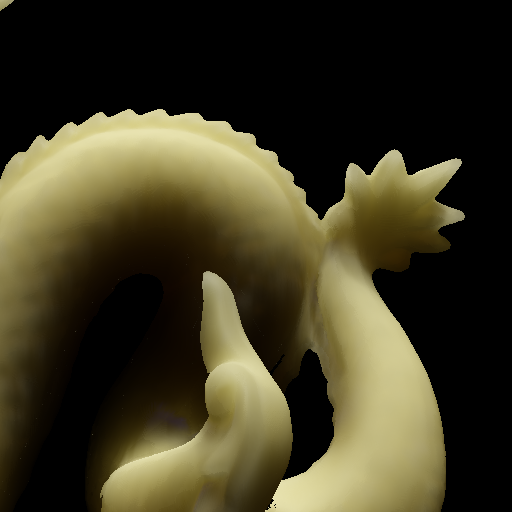
\includegraphics[width=0.4 \linewidth]{images/results/mipmapsc.png}
}
\caption{Detail of a potato Dragon in the first frame of the computation for different mipmap levels. We can see that the second mipmap level is very close to the final result. However, some artifacts due to the stretching of the mipmap appear, such as black spots and bright seams. All the Figures use $N = 32$ and $M = 300$.}
\label{fig:mipblurring}
\end{figure}
\FloatBarrier

\subsection{Environment map illumination}

All the given consideration so far are the same irregardless if we have an environment map or a single directional light. In this section we present the results obtained we environment light illumination. Visually, we obtain a nice result. Obviously, since the samples are split between different lights, an overlapping is inevitable, and we need an higher number of samples to obtain a decent result. The Bunny in Figure \ref{fig:Bunnyenv1} was obtained using 16 directional lights, sampled using the method in \ref{sec:envenv} and \ref{sec:env}, with $N = 80$ (5 samples per light) and $M = 1000$. 

As for reference, we compared our results to the reference image of the potato Buddha from \cite{IMM2013-06646} in Figure \ref{fig:pathBuddhaenv}. We had to try to match the light settings and the camera, but here as well we notice the same color shift as for directional lights. Also in this case we used 16 directional lights to represent our skybox.

\begin{figure}[!h]
\centering
\includegraphics[width=0.7 \linewidth]{images/results/Bunny_env_80_1000_nobias.png}
\caption{Marble Bunny rendered in the Doge environment map. Note that the light is predominantly from the up direction.}
\label{fig:Bunnyenv1}
\end{figure}

%\begin{figure}
%\centering
%\subfloat[{Grace Cathedral}]{
%  \includegraphics[width=0.5 \linewidth]{images/results/Bunny_envgrace_80_1000_nobias.png}
%}
%\subfloat[{Pisa Courtyard}]{
%  \includegraphics[width=0.5 \linewidth]{images/results/Bunny_envPISA_80_1000_nobias.png}
%}
%\caption{Marble Bunny rendered in two other environment maps, Grace Catherdal and Pisa Courtyard.}
%\label{fig:Bunnyenv}
%\end{figure}


\begin{figure}
\centering
\subfloat[{$L = 16$, $N = 90$, $M = 1000$}]{
  \includegraphics[width=0.333 \linewidth]{images/results/happy_Buddha_environment_90over16_1000_nobias.png}
}
\subfloat[{$L = 16$, $N = 90$, $M = 320$}]{
  \includegraphics[width=0.333 \linewidth]{images/results/happy_Buddha_environment_90over16_310_nobias.png}
}
\\
\subfloat[{$L = 16$, $N = 90$, $M = 160$}]{
  \includegraphics[width=0.333 \linewidth]{images/results/happy_Buddha_environment_90over16_160_nobias.png}
}
\subfloat[{Hierarchical integration}]{
  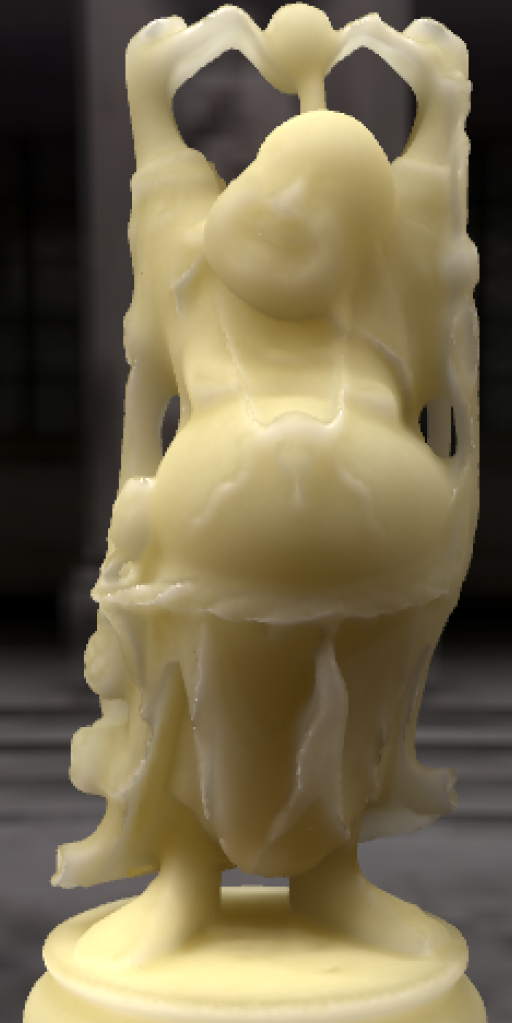
\includegraphics[width=0.333 \linewidth]{images/results/reference_env.png}
}
\caption{Rendering of a potato Buddha using our environment lighting and the Uffizi map.}
\label{fig:pathBuddhaenv}
\end{figure}

\clearpage
In the image of Figure \ref{fig:Dragonenv}, we compare the result using the Pisa Courtyard environment map on a Stanford Dragon, comparing a different number of lights. We can see the more lights we introduce, the more closer we get to a result that approximate true environment illumination. We observe also that the images have more scattering than absorption the more we increase the number of lights: this is because the total number of samples $N$ does not change, so each light has less and less samples available. In this way, the samples tend to concentrate in the center and produce a result where the scattering component is predominant.
\begin{figure}[!h]
\vspace{-0.5cm}
\centering
\subfloat[{2 lights}]{
  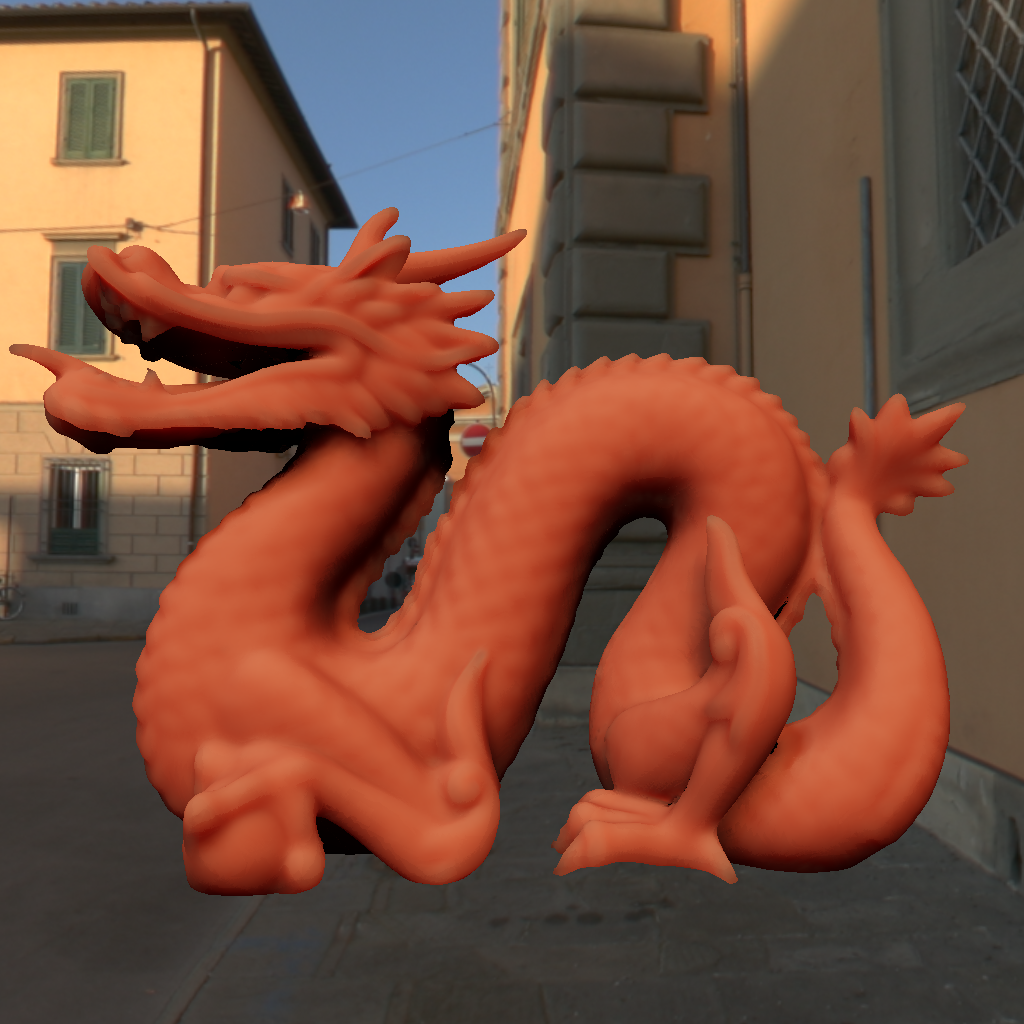
\includegraphics[width=0.4 \linewidth]{images/results/env2.png}
}
\subfloat[{4 lights}]{
  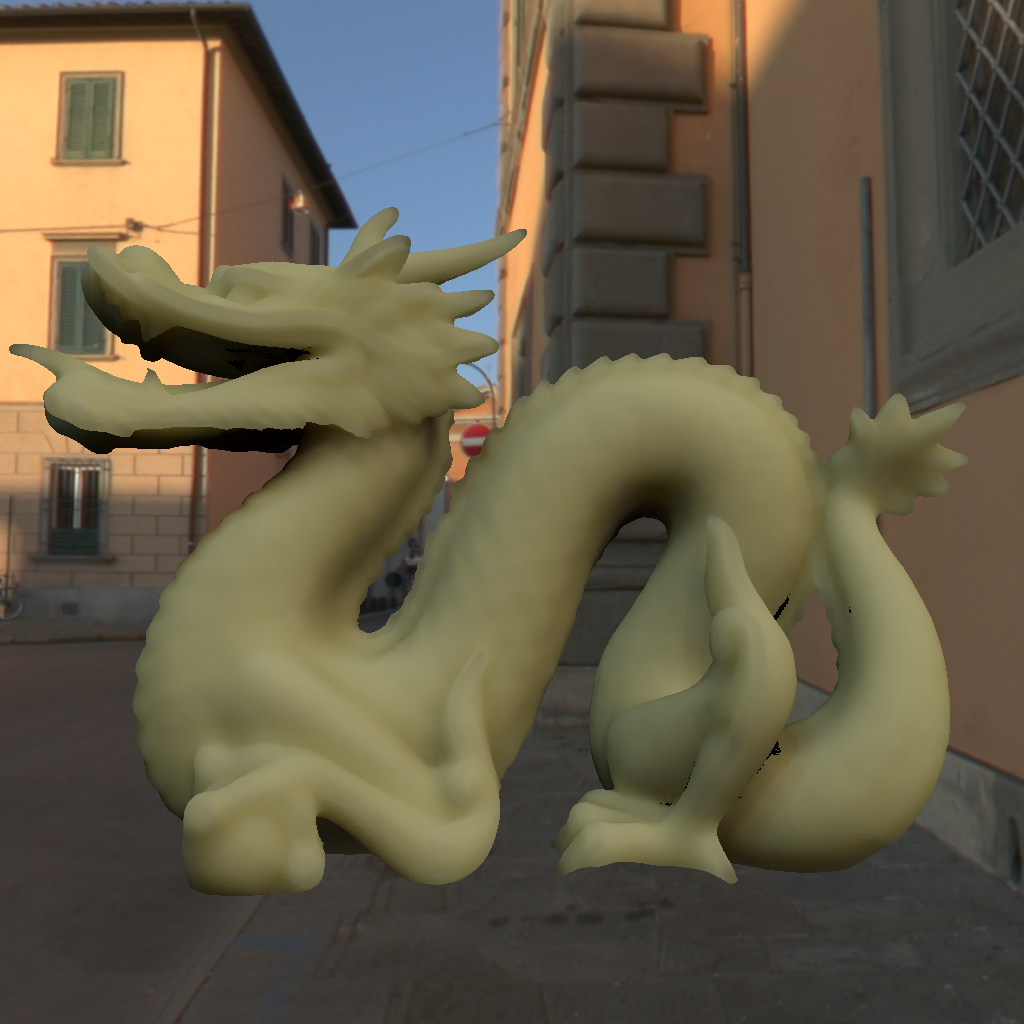
\includegraphics[width=0.4 \linewidth]{images/results/env4.png}
} \\

\subfloat[{8 lights}]{
  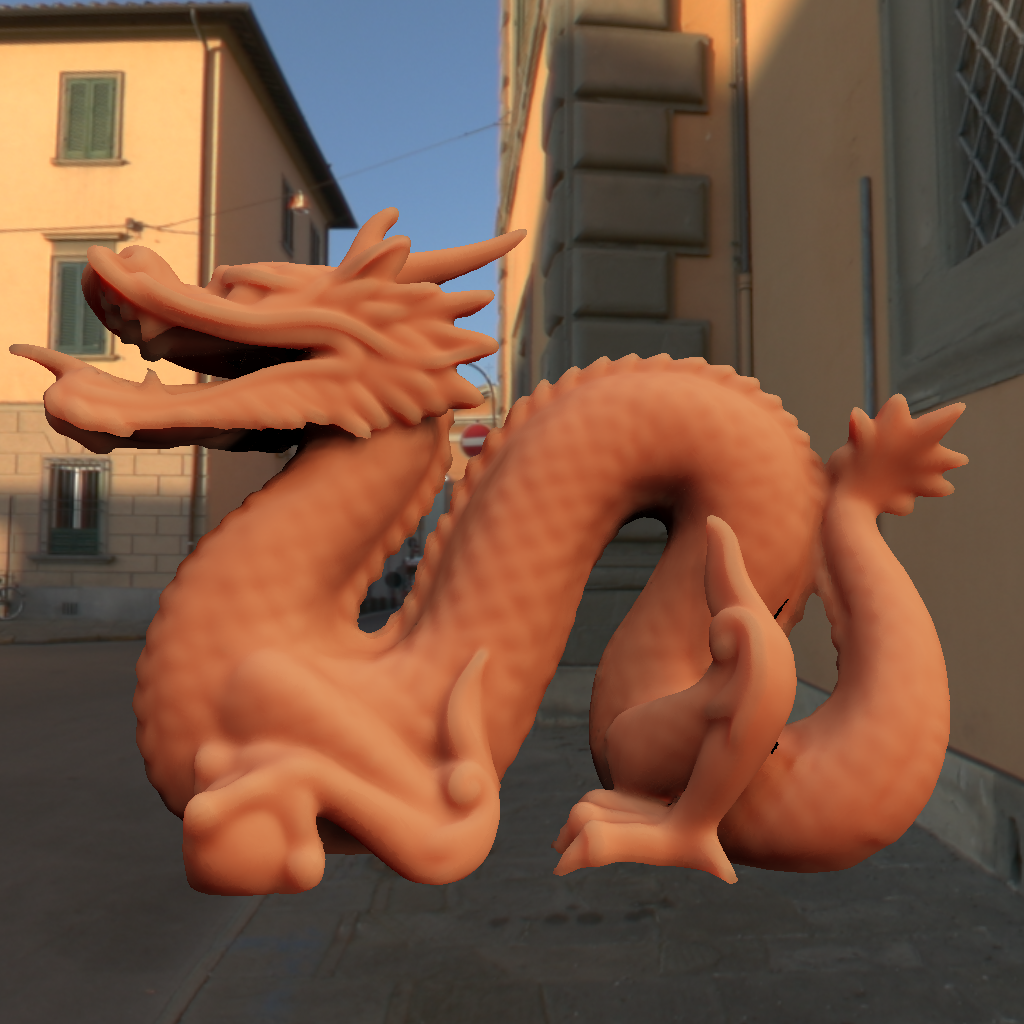
\includegraphics[width=0.4 \linewidth]{images/results/env8.png}
}
\subfloat[{16 lights}]{
  \includegraphics[width=0.4 \linewidth]{images/results/env16.png}
}
\caption{Rendering of a potato Dragon ($N = 32$, $M = 170$) using a different number of directional light to represent the environment map.}
\label{fig:Dragonenv}
\end{figure}

\clearpage
\section{Performance tests}
\label{sec:perf}
In this section, we examine and analyze the performance of our method. The tests in this section were made by keeping in mind the performance requirements we made in chapter \ref{chap:intro}, and they exploit how the different parameters listed in \ref{sec:parameters} influence the final result. For the tests, we used three main models, to which we will refer as Bunny, Dragon and Buddha (see table \ref{table:models}). The models cover a varying range of complexity. The Bunny model represents a typical model used in modern games and consoles ($10^4$ triangles), while the Dragon represents a highly detailed model, usually for visualization purposes ($10^5$ triangles). Finally, the Buddha model represent a high resolution model, and it will be used as a stress test for our algorithm ($10^6$ triangles).

\begin{table}[!ht]
\centering
\begin{tabular}{|l|l|l|}
\hline
Model  & Vertices (\#$V$) & Triangles (\#$\Delta$) \\ \hline
Bunny  & $3581$                                   & $21474 \approx 10^4$                           \\ \hline
Dragon & $50000$                                  & $300000 \approx 10^5$                          \\ \hline
Buddha & $549409$                                 & $3262422 \approx 10^6$                         \\ \hline
\end{tabular}
\caption{The three models used for our tests, with number of vertices and triangles.}
\label{table:models}
\end{table}

All the tests were performed on a NVIDIA GeForce GTX 780Ti, a high-end modern GPU with OpenGL 4.3 capabilities. All the timings measure the average milliseconds during the 20th and the 40th frame during an evolution to convergence of 100 frames. The first frames were not measured because of the overhead introduced by the initialization procedure (texture creation, model parsing and loading, shader compilation, etc.).

\subsection{Time algorithm breakdown}

The first test we are going to perform is to time how much time the algorithm takes to perform the different steps illustrated in chapter \ref{chap:implementation}. When we were timing the algorithm, we divided the whole computation into five different steps:

\begin{enumerate}
	\item Initialization phase, where all the different constants and data structures in the algorithm are created and initialized.
	\item Render to light map step, that corresponds to step 1 in our outline.
	\item Render to radiance map step, that corresponds to step 2 in our outline.
	\item Mipmap generation, as in the extension outlined in section \ref{sec:mipmaps}.
	\item Final render combination, that corresponds to step 3 in our outline.
\end{enumerate}

For this tests we tried all the three models, and the results are shown in Figure \ref{fig:timingssplit}. The parameters were tweaked in order to reach the best compromise between visual quality and performance, in order to measure realistic timings. 

We can observe that, irregardless of the test case, most of the time is spent computing the BSSRDF function for the samples in step 2. Thee render to lightmap step does not have a big performance impact, likely because all the tests were made with one light. We will test in the next section the impact of a different number of lights on the performance.  Another consideration to do is that, as to be expected, the more triangles we have the less samples we can use. As we will see, this is not the only factor that causes a performance drop. However, the big number of triangles that has to be multiplied by the number of directions generates a big load on the GPU for rasterization procedures. 

Regarding the mipmap generation, as expected its performance is not tied to the size of the model, but only to the size of the radiance map texture $W_s$ and to the number of mipmaps we generate. Finally, the final combination step is tied as well to the size of the model, rising slightly with an increasing model size. However, in this case we are rendering only once the model to the main framebuffer, and not $K$ times as in step 2.

\begin{figure}
\centering
\subfloat[Beer Bunny, $67.6 ms$. Point light. $N = 180$, $M = 210$, $q = 2$]{
  \includegraphics[width=0.4 \linewidth]{images/results/example2.png}
}
\subfloat[Detailed timings.]{
\begin{tabular}[b]{lllll}
\multicolumn{5}{c}{\includegraphics[width=0.3 \linewidth]{images/matlab/Bunnychart.pdf}}                                                   \\ \hline
\multicolumn{1}{|l|}{RL}   & \multicolumn{1}{l|}{RR}    & \multicolumn{1}{l|}{MG}   & \multicolumn{1}{l|}{FR}   & \multicolumn{1}{l|}{Tot}   \\ \hline
\multicolumn{1}{|l|}{0.20} & \multicolumn{1}{l|}{66.18} & \multicolumn{1}{l|}{0.8} & \multicolumn{1}{l|}{0.44} & \multicolumn{1}{l|}{67.72} \\ \hline
\end{tabular}
}\\
\subfloat[Ketchup Dragon, $62.0 ms$. Directional light. $N = 20$, $M = 180$.]{
  \includegraphics[width=0.4 \linewidth]{images/results/example1.png}
}
\subfloat[Detailed timings.]{
\begin{tabular}[b]{lllll}
\multicolumn{5}{c}{\includegraphics[width=0.3 \linewidth]{images/matlab/Dragonchart.pdf}}                                                   \\ \hline
\multicolumn{1}{|l|}{RL}   & \multicolumn{1}{l|}{RR}    & \multicolumn{1}{l|}{MG}   & \multicolumn{1}{l|}{FR}   & \multicolumn{1}{l|}{Tot}   \\ \hline
\multicolumn{1}{|l|}{1.07} & \multicolumn{1}{l|}{57.59} & \multicolumn{1}{l|}{0.76} & \multicolumn{1}{l|}{2.56} & \multicolumn{1}{l|}{62.04} \\ \hline
\end{tabular}
}\\
\subfloat[Potato Buddha, $98.0 ms$. Point light. $N = 10$, $M = 300$, $q = 1$]{
  \includegraphics[width=0.4 \linewidth]{images/results/example3.png}
}
\subfloat[Detailed timings.]{
\begin{tabular}[b]{lllll}
\multicolumn{5}{c}{\includegraphics[width=0.3 \linewidth]{images/matlab/Buddhachart.pdf}}                                                   \\ \hline
\multicolumn{1}{|l|}{RL}   & \multicolumn{1}{l|}{RR}    & \multicolumn{1}{l|}{MG}   & \multicolumn{1}{l|}{FR}   & \multicolumn{1}{l|}{Tot}   \\ \hline
\multicolumn{1}{|l|}{11.18} & \multicolumn{1}{l|}{83.90} & \multicolumn{1}{l|}{0.86} & \multicolumn{1}{l|}{1.41} & \multicolumn{1}{l|}{98.00} \\ \hline
\end{tabular}
}
\caption{Rendering of different models, and graphs that illustrate how the timings are split into the different phases of the algorithm. All tests use $W_l = W_s = 512$. The acronyms represent RL = Render to lightmap, RR = Render to radiance map, MG = Mipmap Generation and FR = Final Rendering.}
\label{fig:timingssplit}
\end{figure}

\FloatBarrier
\subsection{Tests for varying parameters}
In this section, we will discuss how well our method behaves for changing parameters. From the quality tests before we have learned that the parameters that are related mostly to the quality of the are $N$, $M$, $q$ and to a certain extent $W_s$. The number of directions $K$ is important in order to ensure to cover the whole model, and if we are generating the cameras automatically it cannot be too low. Of the mentioned parametrs, $M$ and $q$ do not directly influence performance, as they are used only at the beginning of the computation in order to distribute the points on the disc. 
 
\textbf{$N$ parameter}\\
We start by discussing $N$. We can see the results for different value of the parameter in the following table:

\begin{table}[!ht]
\centering
\begin{tabular}{p{3cm}l|l|l|l|l|}
\cline{3-6}
                             &      & \multicolumn{4}{c|}{Number of samples ($N$)}                                          \\ \cline{3-6} 
Model                        & \#$\Delta$& \multicolumn{1}{c|}{1} & \multicolumn{1}{c|}{10} & \multicolumn{1}{c|}{50} & \multicolumn{1}{c|}{100} \\ \hline
\multicolumn{1}{|l|}{Bunny}  & $10^4$ & \mycolor{2}.1                  & \mycolor{5}.3                 & \mycolor{19}.8                  & \mycolor{38}.2                 \\ \hline
\multicolumn{1}{|l|}{Dragon} & $10^5$ & \mycolor{12}.5                 & \mycolor{35}.2                  & \mycolor{140}.6                & \mycolor{275}.3                \\ \hline
\multicolumn{1}{|l|}{Buddha} & $10^6$ & \mycolor{96}.7                 & \mycolor{97}.7                  & \mycolor{128}.0                & \mycolor{216}.0                 \\ \hline
\end{tabular}
\caption{Timings in milliseconds of our method for different models and number of samples $N$ (potato material properties). The other parameters were $L = 1$, $W_s = W_l = 512$, $M = 1000$, $K = 16$.}
\end{table}

We tested $N$ in the range $1-100$. The test with $N = 1$ was introduced to measure the baseline performance of the method (where the most expensive operation is the generation of the random number for the rotation). We did not use zero samples because otherwise the shader compiler optimizations would have removed the base code as well, making the results not significant.

We note that from the graph the time to render the Dragon with 50 samples is slower that rendering the Buddha with the same parameters, despite the Buddha having 10 times the triangles as the Dragon. This suggests that $N$ and the triangle size of the model are not the only factors involved in the performance. Since the heavy computational step is made on a fragment shader in step 2, the number of pixels involved in the computation matters: the Buddha on average occupies less texture area on the directional cameras, and thus the number of computations performed in total is less that the ones for the Dragon. For a low number of samples, the performance is bound by the rasterization time, so the Dragon outperforms the Buddha in this case because of the fewer number of triangles. 

We tested this changing performance according to the area in the following test: we kept the same settings for the directional cameras, but we tried different Dragon sizes. By size, we mean the size of the Dragon using a different scaling transform matrix.

\begin{table}[!ht]
\centering
\begin{tabular}{p{3cm}l|l|l|l|l|}
\cline{3-6}
                             &      & \multicolumn{4}{c|}{Size of the model (units)}                                          \\ \cline{3-6} 
Model                        & \#$\Delta$& \multicolumn{1}{c|}{1} & \multicolumn{1}{c|}{0.5} & \multicolumn{1}{c|}{0.25} & \multicolumn{1}{c|}{0.125} \\ \hline
\multicolumn{1}{|l|}{Dragon}  & $10^5$ & \mycolor{142}.1                  & \mycolor{74}.3                 & \mycolor{34}.9                  & \mycolor{15}.4                 \\ \hline
\end{tabular}
\caption{Timings in milliseconds of our method for different model size (potato material properties). The size of the camera is 2 units, and the model is 2 units wide. The camera does not scale with the model. The other parameters were $N = 50$, $L = 1$, $W_s = W_l = 512$, $M = 1000$, $K = 16$.}
\end{table}

The Dragon, by changing size, occupies a different area of the camera, and so the algorithm performs differently according to the Dragon size. A degrading in quality of the final result is also visible, because of the less number of pixels involved. This problem should be addressed in an eventual extension to the implementation, that should account for these problems in a optimal camera placement.

\textbf{$W_s$ parameter}\\
The next test we performed was on the size of the radiance map. 

\begin{table}[!ht]
\centering
\begin{tabular}{p{3cm}l|l|l|l|l|}
\cline{3-5}
                             &      & \multicolumn{3}{c|}{Size of the radiance map ($W_s$)}                                          \\ \cline{3-5} 
Model                        & \#$\Delta$& \multicolumn{1}{>{\centering\arraybackslash}p{1.2cm}|}{256} & \multicolumn{1}{>{\centering\arraybackslash}p{1.2cm}|}{512} & \multicolumn{1}{>{\centering\arraybackslash}p{1.2cm}|}{1024} \\ \hline
\multicolumn{1}{|l|}{Bunny}  & $10^4$ & \mycolor{11}.4                  & \mycolor{20}.0                 & \mycolor{39}.0                               \\ \hline
\multicolumn{1}{|l|}{Dragon} & $10^5$ & \mycolor{75}.4                 & \mycolor{142}.1                  & \mycolor{299}.4                             \\ \hline
\multicolumn{1}{|l|}{Buddha} & $10^6$ & \mycolor{98}.2                 & \mycolor{127}.0                  & \mycolor{258}.2                             \\ \hline
\end{tabular}
\caption{Timings in milliseconds of our method for different models and size of the radiance map $W_s$ (ketchup material properties). The other parameters were $N = 50$, $L = 1$, $W_l = 512$, $M = 1000$, $K = 16$.}
\label{table:sizews}
\end{table}

As we can see from table \ref{table:sizews}, the performance scales linearly with the radiance map size. This means that if we double the size of the radiance map, the time to render the model roughly doubles. This comes from the fact that most of the time in the computation is spent in rendering to the radiance map, that is a pixel bound operation. So if we double the size of map, we roughly double the number of pixels involved and thus the number of the fragment shader invocations in step 2. 

\textbf{$K$ parameter}\\
The next test is about the number of directions used to render the model, $K$.

\begin{table}[!ht]
\centering
\begin{tabular}{p{3cm}l|l|l|l|l|}
\cline{3-6}
                             &      & \multicolumn{4}{c|}{Number of directions ($K$)}                                          \\ \cline{3-6} 
Model                        & \#$\Delta$& \multicolumn{1}{c|}{4} & \multicolumn{1}{c|}{8} & \multicolumn{1}{c|}{16} & \multicolumn{1}{c|}{32} \\ \hline
\multicolumn{1}{|l|}{Bunny}  & $10^4$ & \mycolor{6}.6                  & \mycolor{10}.0                 & \mycolor{20}.1                  & \mycolor{42}.1                 \\ \hline
\multicolumn{1}{|l|}{Dragon} & $10^5$ & \mycolor{36}.7                 & \mycolor{70}.1                  & \mycolor{143}.0                & \mycolor{306}.2               \\ \hline
\multicolumn{1}{|l|}{Buddha} & $10^6$ & \mycolor{32}.5                 & \mycolor{55}.8                  & \mycolor{128}.3                & \mycolor{363}.5                 \\ \hline
\end{tabular}
\caption{Timings in milliseconds of our method for different models and different number of directions $K$ (ketchup material properties). The other parameters were $N = 50$, $L = 1$, $W_s = W_l = 512$, $M = 1000$, $q = 1$.}
\end{table}

We can see that the performance for the models scales linearly. We can see from this test that is a big advantage to place the cameras manually, instead of relying on an automatic algorithm. A careful placement of the cameras can cover the whole model evenly with a smaller number of cameras that an automatic placement. In our implementation, we needed to use at least 16 cameras to ensure that most of the models were covered. On the other hand, with careful placement of the cameras, we were able to lower the number of cameras up to 8 in all cases, thus doubling the performance. Also in this test, we can see that the minor area occupation of the Buddha improves its performance for 4,8, and 16 directions. For 32 directions, the number of triangles that actually need to be rasterized ($32 \cdot 10^6$) probably becomes so high that memory issues on the GPU become important.

\textbf{Different types of lights}\\
We tested the different times in performance for different kind of lights. Since the operations performed are roughly the same (the point light requires an extra division), also is the performance:

\begin{table}[!ht]
\centering
\begin{tabular}{p{3cm}l|l|l|l|}
\cline{3-5}
                             &      & \multicolumn{3}{c|}{Type of light}                                          \\ \cline{3-5} 
Model                        & \#$\Delta$& \multicolumn{1}{c|}{Point light} & \multicolumn{1}{c|}{Directional light}  & \multicolumn{1}{c|}{No loop} \\ \hline
\multicolumn{1}{|l|}{Dragon}  & $10^5$ & \mycolor{61}.8                  & \mycolor{60}.3                            & \mycolor{60}.1                 \\ \hline
\end{tabular}
\caption{Timings in milliseconds of our method for different types of light (potato material properties), one light. The other parameters were $N = 20$, $W_s = W_l = 512$, $M = 1000$, $K = 16$.}
\end{table}

We times a third case, that is when we strip the outer loop in listing \ref{lst:multi}, thus obtaining a shader suitable for only one light. In this case, we can see that the performance slightly improves by fractions of a millisecond.

\textbf{Different materials}\\
We finally tried to see if different materials gave a different performance on the method. As we expected, the material does not influence the rendering time, as the computations in the BSSRDF do not actually take advantage on the material type to easy any computation. We can see the test result in the following table:
\begin{table}[!ht]
\centering
\begin{tabular}{p{3cm}l|l|l|l|l|}
\cline{3-6}
                             &      & \multicolumn{4}{c|}{Material}                                          \\ \cline{3-6} 
Model                        & \#$\Delta$& \multicolumn{1}{c|}{Ketchup} & \multicolumn{1}{c|}{Beer} & \multicolumn{1}{c|}{White grapefruit} & \multicolumn{1}{c|}{Potato} \\ \hline
\multicolumn{1}{|l|}{Dragon}  & $10^5$ & \mycolor{61}.7                  & \mycolor{61}.6                 & \mycolor{62}.0                 & \mycolor{62}.1                 \\ \hline
\end{tabular}
\caption{Timings in milliseconds of our method for different materials. The other parameters were $N = 20$, $L = 1$, $W_s = W_l = 512$, $M = 300$, $K = 16$.}
\end{table}

\clearpage
\subsection{Tests on environment lighting}
The considerations so far discussed apply also in environment map lighting, that we converted to a certain number $L$ of directional lights. So discussing the impact on performance of multiple lights and the impact of environment lighting is essentially the same, apart from a initialization delay to generate the lights from the environment map that we will not consider.

The timings for different kind of lights are reported in the following table:
\begin{table}[!ht]
\centering
\begin{tabular}{p{3cm}l|l|l|l|l|l|}
\cline{3-7}
                             &                      & \multicolumn{5}{c|}{Number of lights $L$}                                                             \\ \cline{3-7} 
Model                        & \#$\Delta$ & \multicolumn{1}{c|}{1} & \multicolumn{1}{c|}{2} & \multicolumn{1}{c|}{4} & \multicolumn{1}{c|}{8} &  \multicolumn{1}{c|}{16} \\ \hline
\multicolumn{1}{|l|}{Dragon}  & $10^5$ & \mycolor{96}.6                 & \mycolor{98}.0                 & \mycolor{100}.0                 & \mycolor{103}.8           & \mycolor{110}.5      \\ \hline
\end{tabular}
\caption{Timings in milliseconds of our method for different number of lights (environment map approximation, material properties for potato). The other parameters were $N = 32$, $W_s = W_l = 512$, $M = 300$, $K = 16$.}
\label{table:multilightenvDragon}
\end{table}
\vspace{-0.2cm}
As we can see, even if we maintain the same number of samples ($N = 32$, so the number of samples per light changes) the performance worsen increasing the number of lights. To look at this into more detail, we broke down the timings again in the different steps. We can see in Figure \ref{fig:numblights} that the increase in timing is due to step 1, the render to lightmap: in fact, we have to render the model once for each light, that implies a performance penalty.

\begin{figure}[!ht]
\centering
  \includegraphics[width=0.8\linewidth]{images/matlab/multiple_lights_test.pdf}

\caption{Rendering times for the environment lighting of Figure \ref{table:multilightenvDragon}, split into the various components. The rendering times of step 2 are not shown, but they are $[91.8\ 93.3\ 93.5\ 95.0\ 97.1]$.}
\label{fig:numblights}
\end{figure}
